%% LyX 1.6.5 created this file.  For more info, see http://www.lyx.org/.
%% Do not edit unless you really know what you are doing.
\documentclass[11pt, spanish]{article}
\usepackage{helvet}
\renewcommand{\familydefault}{\sfdefault}
\usepackage[T1]{fontenc}
\usepackage[utf8]{inputenc}
%\usepackage[latin9]{inputenc}
\usepackage{subfigure}
\usepackage{listings}
\usepackage{array}
\usepackage{textcomp}
\usepackage{graphics}
\usepackage{graphicx}
\usepackage{anysize}
\usepackage{url}
\usepackage[tikz]{bclogo}



\makeatletter



%%%%%%%%%%%%%%%%%%%%%%%%%%%%%% LyX specific LaTeX commands.
%% Because html converters don't know tabularnewline
\providecommand{\tabularnewline}{\\}

%%%%%%%%%%%%%%%%%%%%%%%%%%%%%% Textclass specific LaTeX commands.
\newenvironment{lyxcode}
{\par\begin{list}{}{
\setlength{\rightmargin}{\leftmargin}
\setlength{\listparindent}{0pt}% needed for AMS classes
\raggedright
\setlength{\itemsep}{0pt}
\setlength{\parsep}{0pt}
\normalfont\ttfamily}%
 \item[]}
{\end{list}}

\makeatother

\usepackage{babel}
\addto\shorthandsspanish{\spanishdeactivate{~<>}}

\usepackage[a4paper,left=25mm,right=25mm,top=25mm, bottom=25mm]{geometry}
%\marginsize{3cm}{3cm}{2.75cm}{2.5cm}
\definecolor{mycolor}{RGB}{255, 245, 213}

\renewcommand{\lstlistingname}{Código}% Listing -> Código


\begin{document}
\begin{center}
{\Large \thispagestyle{empty}}{\large UNIVERSIDAD DE ALCALÁ}{\Large{} }
\par\end{center}{\Large \par}

\begin{center}
Departamento de Automática
\par\end{center}

\begin{center}
Grado en Ingeniería Informática

\par\end{center}

\vspace{6cm}

\begin{center}
{\LARGE Práctica 2: Herramientas de desarrollo y\\ Servicios POSIX para la gestión de procesos}
\par\end{center}{\LARGE \par}
\vspace{11cm}


\begin{center}
{\large Sistemas Operativos}
\par\end{center}{\large \par}


\newpage{}
$\ $
\thispagestyle{empty} % para que no se numere esta pagina
\newpage{}
\tableofcontents{}
\newpage{}


\section{Competencias asociadas a la práctica}
\begin{enumerate}

\item Distinguir las funcionalidades implementadas en una \textit{shell} completa de Unix y las funcionalidades implementadas en el intérprete de órdenes de la práctica y lo que esto implica respecto a los resultados obtenidos al ejecutar diversas órdenes en ambos casos.


\item Identificar los servicios POSIX de gestión de procesos necesarios para la ejecución de órdenes concretas, internas y externas (en primer y segundo plano).

%\item Completar diferentes fragmentos de código relacionados con el funcionamiento de los servicios POSIX de comunicación de procesos (servicios POSIX de \textit{pipes} y señales). 

\item Programar el ciclo de ejecución del intérprete de órdenes. 

\item Programar la ejecución de órdenes internas del intérprete de órdenes.

\item Programar la ejecución en primer plano de órdenes externas del intérprete de órdenes.
% he quitado simples porque al final debería funcionar simple o compuesta en primer plano o en segundo plano

\item Programar la ejecución en segundo plano de órdenes externas del intérprete de órdenes. 

\item Programar el uso de redirecciones de entrada y salida estándar ($>$, $<$) en el intérprete de órdenes.

\item Programar el uso de las tuberías sin nombre en el intérprete de órdenes.

\item Programar la secuencia de órdenes (órdenes separadas por ‘;’) en el intérprete de órdenes.

\item Aplicar las herramientas de desarrollo clásicas en Unix: \texttt{gcc}, \texttt{make}, \texttt{gdb} y uso de bibliotecas estáticas.

\item Utilizar un estilo de programación (documentación incluida) correcto y uniforme en la programación del intérprete de órdenes.

%\item Programar mejoras en el intérprete solicitado relacionadas con la simplificación de código, completitud de funcionalidades u otras ideas creativas.
\item Desarrollar un proyecto en equipo.

%Demostrar creatividad y actitud proactiva en relación con el intérprete solicitado (simplificación de código, completitud de funcionalidades u otras ideas creativas.

%\item Valorar de manera justificada y ética la participación de los compañeros al equipo en el proyecto desarrollado (actitud: perseverancia, responsabilidad, asistencia, capacidad de colaboración, capacidad de organización, de liderazgo y de resolución de conflictos).

\end{enumerate}


\section{Introducción}

En prácticas anteriores el alumno se ha iniciado en el uso de un intérprete de órdenes, \textit{bash}, como interfaz de usuario en Linux. 

Esta práctica tiene como objetivo principal introducir al alumno en la interfaz de aplicaciones, comenzando con el uso, a alto nivel, de las llamadas al sistema (en concreto, servicios POSIX) para gestionar procesos y su comunicación, y en menor medida, llamadas al sistema, o más bien, servicios POSIX, para gestión de archivos, como preámbulo a su estudio exhaustivo en la asignatura de Sistemas Operativos Avanzados, de segundo curso de los grados de Ingeniería Informática e Ingeniería de Computadores. 

Para lograr el objetivo previo, el alumno aplicará los conceptos vistos en las clases teóricas y en el laboratorio mediante la implementación parcial de un intérprete de órdenes en Unix (al que denominaremos \textit{minishell}). 

Otro objetivo principal de esta práctica es que el alumno sea capaz de usar las herramientas de desarrollo clásicas utilizadas en entornos Unix, tal y como se han descrito también en las clases teóricas. Actualmente existen entornos de desarrollo (o IDEs) muy avanzados, tales como \textit{Eclipse}, \textit{Netbeans}, etc., que abstraen al desarrollador
de casi todos los detalles relacionados con la compilación del proyecto, de
manera que su productividad aumenta al permitir que se concentre en la creación de código. Esta perspectiva, a pesar de ser la empleada comúnmente en entornos profesionales,
presenta dos problemas: por una parte esa abstracción impide conocer qué sucede
en el proceso de compilación a bajo nivel y, por otra parte, ese desconocimiento reduce la 
capacidad de resolver problemas que pudieran surgir.


Hablar de programación bajo Unix es hablar de C. Este lenguaje de  programación se creó con el único objetivo
de recodificar Unix (que en sus orígenes estaba programado en ensamblador) en
un lenguaje de alto nivel, decisión que, por cierto, fue revolucionaria
en su época. Además, todo el desarrollo de Arpanet y su sucesora, Internet,
se basó en la utilización de máquinas Unix. Por lo tanto, C ha tenido un impacto
decisivo en el desarrollo de la informática, hasta el punto de que la práctica
totalidad de los lenguajes más extendidos en la actualidad 
(Java, C++, C\# o PHP, entre otros) han tomado elementos de C, o directamente
son una evolución del mismo. Así pues, no es de sorprender que Unix y C
tengan una relación más que estrecha, y por este motivo no se pueda abordar
el estudio de Unix sin utilizar C.

Adicionalmente, un subobjetivo importante dentro de la práctica es acostumbrar al
alumno a trabajar en equipo, una cualidad fundamental de cara al mundo
laboral. Este hecho implica realizar un diseño adecuado de las aplicaciones,
su modularización, así como una buena metodología de desarrollo y comunicación
dentro del equipo\footnote{En equipos de desarrollo profesionales, se suele utilizar la ayuda
de sistemas de control de versiones como CVS o Subversion. Es un software
imprescindible que permite que varias personas trabajen simultáneamente
sobre un mismo código, manteniendo un registro de cambios.}.

%Una parte de la práctica se realiza conjuntamente, y corresponde
%a la parte comn que necesitan todos los módulos, mientras que cada
%módulo se asignar a una persona y se desarrollará individualmentea\footnote{En equipos de desarrollo profesionales, se suele utilizar la ayuda
%de sistemas de control de versiones como CVS o Subversion. Es un software
%imprescindible que permite que varias personas trabajen simultneamente
%sobre un mismo código, manteniendo un registro de cambios.%
%}.

\section{Ciclo de creación de un programa}

Como en cualquier otro entorno, crear un programa bajo UNIX requiere una
serie de pasos, que deben ser ya de sobra conocidos por el
alumno:

% (ver figura~\ref{cap:ciclo}).

%\begin{figure}
%\begin{centering}
%\includegraphics[scale=0.5]{figs/ciclo.eps}
%\par\end{centering}

%\caption{\label{cap:ciclo}Ciclo de desarrollo.}

%\end{figure}

\begin{itemize}
\item {
\textit{Creaci\'on y edici\'on} del programa o \textbf{c\'odigo fuente} sobre un
archivo de texto, empleando para ello una herramienta denominada
\textbf{editor}. En caso de programar en lenguaje C, el convenio es que
dicho archivo tenga extensi\'on ``\texttt{.c}''.}
\item {
\textit{Compilaci\'on} del c\'odigo fuente mediante otra herramienta denominada
\textbf{compilador}, gener\'andose un \textbf{archivo objeto},
que en UNIX suele tener extensi\'on
``\texttt{.o}''. A veces, en lugar de generarse el
archivo objeto directamente se genera un archivo intermedio en
ensamblador (en UNIX t\'ipicamente con extensi\'on
``\texttt{.s}'') que, a continuaci\'on, es necesario
ensamblar con un \textbf{ensamblador} para obtener el archivo
objeto. Adem\'as, en C existe una etapa previa a la compilaci\'on en la
que el archivo fuente pasa por otra herramienta denominada
\textbf{preprocesador}.}
\item {
\textit{Enlazado} del archivo objeto con otros archivos objeto necesarios, as\'i
como con las bibliotecas que sean necesarias para as\'i obtener el
\textbf{archivo de programa ejecutable}. Esta labor es llevada a cabo
por un programa denominado \textbf{enlazador}.}
\item {
Finalmente, \textit{ejecutar} el programa tal cual o, en caso de ser
necesario, \textit{depurar} el programa con una herramienta denominada
\textbf{depurador} o \textit{debugger}. Si se detectan problemas en la ejecución,
ser\'a necesario editar el programa fuente y corregir los fallos,
reinici\'andose el ciclo de desarrollo hasta obtener un programa sin
errores.}
\end{itemize}

El proceso anterior queda ilustrado con un ejemplo en la Figura \ref{fig:compilacion}.
En un sistema Linux, como el empleado en el laboratorio, las herramientas
cl\'asicas encargadas de cada etapa son las siguientes:
%
%\newpage
\begin{figure}[ht!]
\begin{centering}
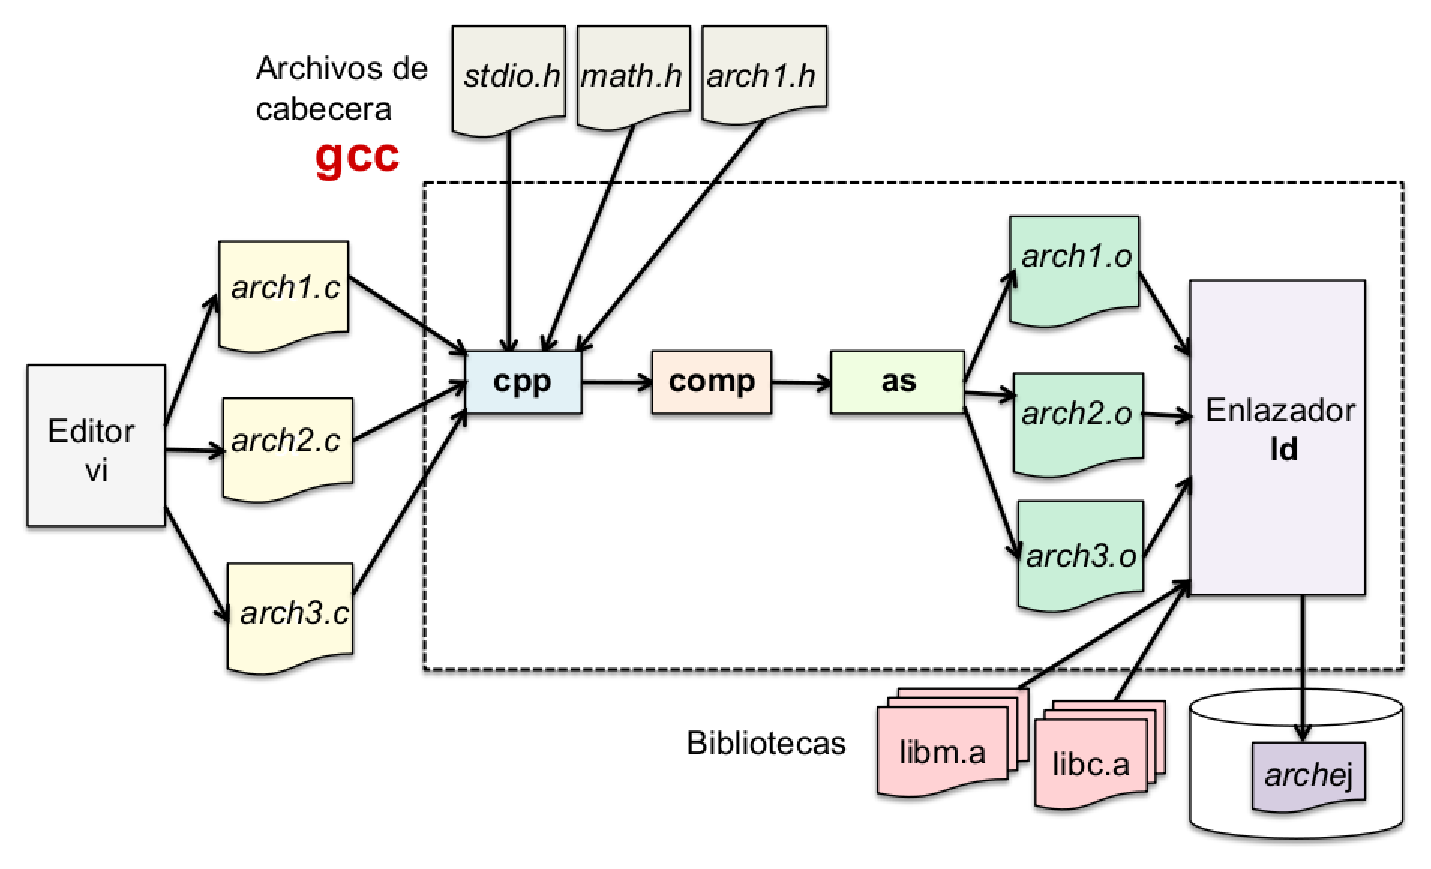
\includegraphics[scale=0.53]{figs/compilacionvariosmodulosUnix}
\par\end{centering}

\caption{\label{fig:compilacion}Ejemplo de generación de un archivo ejecutable en lenguaje C.}

\end{figure}

\begin{itemize}
\item {
\textbf{Editor}: existe gran variedad de ellos, siendo los m\'as populares
\texttt{\textbf{emacs}} y \texttt{\textbf{vi}}. En el laboratorio se
recomienda el uso del editor \texttt{\textbf{vi}}, o, si se prefiere, un editor en modo gr\'afico.}
\item {
\textbf{Preprocesador}, \textbf{compilador}, \textbf{ensamblador}, y \textbf{enlazador}: estas herramientas
pueden encontrarse de forma individual, pero en un sistema Linux
t\'ipicamente encontramos la herramienta \texttt{\textbf{cc}}
(realmente la herramienta que invoca la compilación en C y C++ de GNU, \texttt{gcc}), que
se encarga de llamar al preprocesador, compilador, ensamblador, y enlazador, seg\'un se necesiten. En cualquier caso, y
aunque por lo general no las utilizaremos de forma individual, las
herramientas son:}

\begin{itemize}
\item {
Preprocesador: \texttt{cpp}.}
\item {
Compilador: \texttt{comp}.}
\item {
Ensamblador: \texttt{as}.}
\item {
Enlazador: \texttt{ld}.}
\end{itemize}

\item {\textbf{Depurador}: el depurador por excelencia en el entorno Linux (y en UNIX en
general) es \texttt{gdb}.}
\end{itemize}

Vamos a analizar cada fase con más detalle.

\subsection{Edici\'on del archivo fuente}

La edición del código fuente se puede realizar con cualquier programa capaz de
editar archivos en texto plano. Por su amplia difusión, gran versatilidad y
velocidad de edición se utiliza mucho el editor \texttt{vi}, o versiones gráficas como \texttt{gvim}. 

El editor \texttt{vi} es mucho m\'as potente y r\'apido que los
editores t\'ipicos de MS{}-DOS o Windows, como el \texttt{Bloc de Notas} o
el \texttt{edit}, y otros editores de entorno de
ventanas, como \texttt{gedit}\footnote{El uso de
\texttt{vi} al principio puede ser un poco frustrante por lo
que, si el alumno no conoce el manejo de esta herramienta, es
recomendable seguir alguno de los tutoriales existentes como, por ejemplo, el proporcionado en el Aula Virtual de la  UAH, en concreto, en el espacio virtual reservado para la asignatura.}.

La forma de editar el programa ser\'a:

\begin{lyxcode}
user@host:\$ vi programa.c
\end{lyxcode}

Para salir del editor hay que pulsar escape y posteriormente teclear ``:q!'' si no se desea guardar los cambios, o bien ``:wq'' si se quieren guardar los cambios.

\subsection{Compilaci\'on y enlazado}

El programa \texttt{gcc} es el encargado de compilar, enlazar y
generar el archivo ejecutable a partir del archivo fuente. La forma
m\'as sencilla de invocarlo es  la siguiente:

\begin{lyxcode}
user@host:\$ gcc programa.c
\end{lyxcode}

Esta orden preprocesa, compila, ensambla y enlaza, generando el archivo
de salida ejecutable \texttt{a.out}. T\'ipicamente no se desea que esto sea as\'i, por lo que se emplea la opci\'on
\texttt{-o} para establecer el nombre del archivo generado:

\begin{lyxcode}
user@host:\$ cc programa.c {}-o programa
\end{lyxcode}

Para ejecutar el programa es necesario invocarlo de la forma siguiente:

\begin{lyxcode}
user@host:\$ ./programa
\end{lyxcode}

Es necesario el empleo del \texttt{./} antes del nombre de
programa para indicarle al int\'erprete de \'ordenes que el programa
reside en el directorio actual de trabajo (\texttt{.}).  En caso de no especificarlo, s\'olo se buscar\'ia el programa en
aquellos directorios del sistema especificados en la variable de
entorno \texttt{PATH}.

\begin{lyxcode}
user@host:\$ echo \$PATH
/usr/local/bin:/usr/bin:/bin:/usr/bin/X11:/usr/games
\end{lyxcode}

El programa \texttt{gcc} es muy flexible y soporta
una gran cantidad de opciones que le permiten, por ejemplo, detenerse
tras un determinado paso del proceso (por ejemplo, de la compilaci\'on)
o aceptar varios archivos de entrada incluso de diferentes tipos
(fuente, objeto o en ensamblador), siendo capaz de procesar cada uno de
ellos de la manera adecuada para generar el archivo de salida que se le
pide.

Por ejemplo, la siguiente orden compila el archivo
\texttt{programa.c} y el objeto resultante lo enlaza con el
objeto \texttt{funciones.o}, dando como resultado el programa
de nombre \texttt{programa}:

\begin{lyxcode}
user@host:\$ gcc programa.c funciones.o -o programa
\end{lyxcode}

La siguiente orden compila los archivos fuente indicados, generando los
archivos objeto de cada uno de ellos pero no contin\'ua con el enlazado
y generaci\'on del ejecutable final:

\begin{lyxcode}
user@host:\$ gcc -c programa.c funciones.c
\end{lyxcode}

A continuaci\'on se muestra un resumen de las opciones m\'as frecuentes
con las que se suele invocar \texttt{gcc}.

\begin{center}
\begin{tabular}{|c|p{10.7cm}|}
\hline 
\textbf{Opción} & \textbf{Descripción} \tabularnewline
\hline
\hline 
{}\texttt{-E} & Parar tras el preprocesado.\tabularnewline
\hline 
{}\texttt{-S} & Parar tras el compilado (no ensamblar).\tabularnewline
\hline 
{}\texttt{-c} & Parar antes de enlazar.\tabularnewline
\hline
{}\texttt{-o} nombre & Especificar el nombre del archivo de salida.\tabularnewline
\hline
{}\texttt{-g} & Incluir información de depuración.\tabularnewline
\hline
{}\texttt{-Wall} & Mostrar todos los avisos de compilación.\tabularnewline
\hline
{}\texttt{-pedantic} & Comprobar que el programa es C estándar.\tabularnewline
\hline
{}\texttt{-On} & Grado de optimización de código, donde $n$ es un entero desde $n=0$ (ninguna) a $n=3$ (máxima).\tabularnewline
\hline
{}\texttt{-D macro[=valor]} & Definir una macro (\texttt{\#define}) y su valor ($1$ si se omite).\tabularnewline
\hline
{}\texttt{-I directorio} & Indica un directorio en donde buscar archivos de cabecera (\texttt{.h}).\tabularnewline
\hline
{}\texttt{-L directorio} & Indica un directorio donde buscar bibliotecas compartidas.\tabularnewline
\hline
{}\texttt{-lbiblioteca} & Utilizar la biblioteca compartida \texttt{lbiblioteca.a}.\tabularnewline
\hline
{}\texttt{-static} & Enlazar bibliotecas estáticamente.\tabularnewline
\hline
\end{tabular}
\par\end{center}

\subsection{Depuración}

El depurador est\'andar de UNIX es \texttt{gdb}. Se trata de un
depurador muy potente y extendido en la industria, pero s\'olo admite
una interfaz de l\'inea de \'ordenes que, a priori, puede resultar
engorrosa y dif\'icil de aprender. Existen
{\em front-ends} gr\'aficos para poder trabajar con
\'el de un modo m\'as c\'omodo, como por ejemplo la aplicación \texttt{ddd}.

El uso del depurador es necesario para la r\'apida detecci\'on de
errores en los programas, y por lo tanto debe ser una prioridad para el
alumno. El ahorro de tiempo que conlleva su aprendizaje supera con
mucho el tiempo perdido en perseguir errores dif\'iciles de localizar
de forma visual o mediante el uso de otras ``t\'ecnicas'' de
depuraci\'on como sembrar los programas de llamadas a
\texttt{printf()}.

Como material de apoyo de la pr\'actica se ha incluido un breve tutorial
sobre el uso de \texttt{gdb} en la asignatura de Sistemas Operativos,  en el Aula Virtual de la UAH.

La mejor depuración es la que no es necesario hacer. Para ello
se puede recurrir a muchos ``trucos'' que se aprenden con la experiencia,
como desarrollar de manera incremental, añadiendo poco a poco funciones 
a nuestro programa, verificar la corrección de cada funcionalidad nueva,
abordar un único problema a la vez, etc. Las actividades
propuestas en esta práctica están pensadas en esta línea; 
se sugiere observar cómo se aborda la construcción de los programas.

\section{Automatización del proceso de desarrollo de aplicaciones: \texttt{make}}


El desarrollo de un programa es una actividad c\'iclica en la que puede
ser necesario recompilar muchas veces m\'ultiples archivos fuente
dependientes unos de otros, y es posible que necesitemos usar
m\'ultiples opciones en l\'inea de llamada a \texttt{cc}.
Esto, aparte de la incomodidad, puede ser causa de un desarrollo lento
y sensible a errores.

Para evitarlo en lo posible, en los entornos UNIX suele ser habitual el
uso de la herramienta \texttt{make} para automatizar las
reconstrucciones del c\'odigo y minimizar el tiempo de compilación. Para ello, s\'olo es necesario crear un
archivo llamado \texttt{Makefile}, que especifica la forma en
que deben construirse los objetos, ejecutables o bibliotecas, y las
dependencias entre ellos. Adem\'as, \texttt{make} tambi\'en es
capaz de hacer otras cosas como ejecutar incondicionalmente conjuntos
de \'ordenes.

El programador novato, por lo general, es reacio a la utilizaci\'on de
esta herramienta, bien porque considera innecesario el uso de
\texttt{make}, bien por pereza a la hora de crear el
\texttt{Makefile}, bien por no dominar su uso. El empleo de
\texttt{make} es requisito para todas las pr\'acticas, y el
alumno podr\'a comprobar de forma palpable la enorme ganancia de tiempo
que conlleva su uso a cambio de unos minutos en la creaci\'on de un
\texttt{Makefile} y el siempre necesario proceso de aprendizaje.

Puede encontrar numerosa documentación en Internet acerca del uso del \texttt{make}\footnote{En la asignatura de Sistemas Operativos, en el Aula Virtual de la UAH, en la sección \textit{Material complementario} de la práctica 3, también se han incluido algunos enlaces de interés para el estudio de la herramienta  \texttt{make}.}.

%\subsection{Automatización de la creación del \textit{Makefile}}

%El proceso de desarrollo de aplicaciones en la vida real suele ser 
%más complejo que el descrito en la práctica. Hay que tener en cuenta
%cuestiones como la portabilidad del código, la disponibilidad de
%determinadas bibliotecas, la instalación del software, su empaquetado,
%y una numerosa cantidad de aspectos que, si bien no son esenciales
%para la ejecución del programa, sí lo son para su utilización práctica. Hacer un archivo \texttt{Makefile} que tenga en cuenta todas las 
%cuestiones previas está lejos de ser trivial, hasta el punto de que sólo
%en aplicaciones sencillas el programador genera manualmente
%dicho archivo. Por esta razón, para realizar estas tareas, se utilizan junto con \texttt{make} otras herramientas para la automatización de la creación de archivos \textit{Makefile} personalizados.\footnote{Herramientas como \texttt{automake}, \texttt{autoconf}, etc., están fuera del ámbito de esta práctica, pero es interesante conocer su existencia para comprender el proceso estándar de compilación de aplicaciones Unix.}


\section{Modelo de los procesos en UNIX}\label{sec:ModeloProcUNIX}

En Unix todo proceso es creado por el núcleo del SO, previa petición
de otro proceso, estableciéndose una relación jerárquica entre el
proceso que realiza la petición de creación, conocido como \textbf{proceso
padre}, y el nuevo proceso, denominado \textbf{proceso hijo}. Un proceso
padre puede tener varios hijos y todo hijo tiene únicamente un padre,
tal y como se puede apreciar en la Figura \ref{cap:Jerarquia}. 

\begin{figure}
\begin{centering}
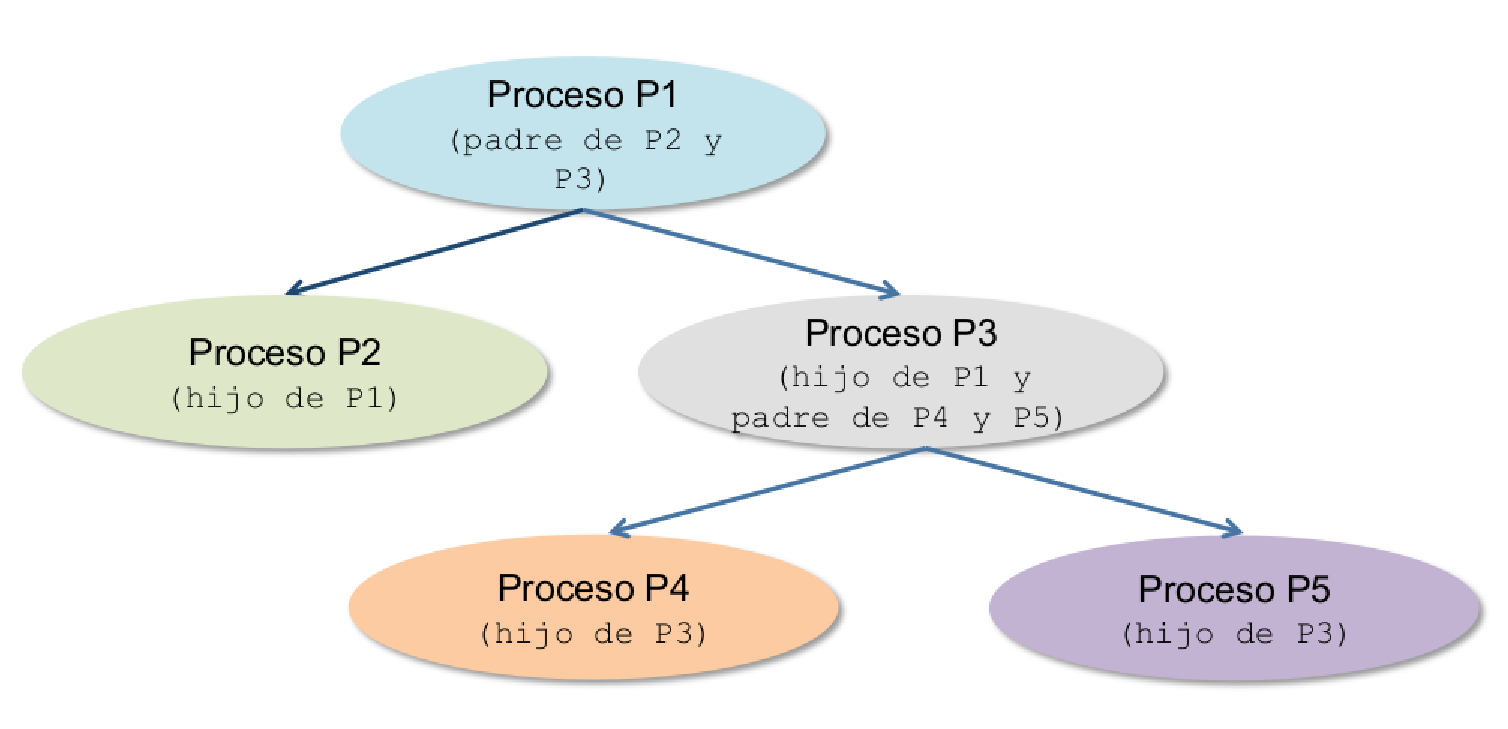
\includegraphics[scale=0.45]{figs/jerarquia_procesos}
\par\end{centering}

\caption{\label{cap:Jerarquia}Jerarquía de procesos en UNIX.}

\end{figure}

Hay una cuestión importante que cabe mencionar: si todo proceso necesita
tener un proceso padre, ¿cuál es el primer proceso del que se originan todos los procesos en UNIX? La respuesta es el proceso \emph{init}, proceso lanzado por el SO durante el arranque del sistema responsable	 de iniciar los procesos necesarios para poder
operar. De hecho, todos los procesos que hay en el sistema descienden
de una manera u otra del proceso \emph{init}. La jerarquía de procesos
existente en una máquina puede consultarse por medio de la orden \texttt{pstree},
si bien no está presente por defecto en todas las instalaciones de
Linux.

Por lo general, en un SO no todos los procesos tienen la misma prioridad.
En el caso de Unix, a cada proceso se le puede asociar una prioridad
distinta. La prioridad es un mecanismo que permite al SO dar un trato
de privilegio a ciertos procesos a la hora de repartir la utilización
de la CPU. Por ejemplo, resultaría poco eficiente asignar la misma
prioridad a un proceso que se ejecuta en {\em background} que a un proceso
interactivo, que tiene a un usuario pendiente de obtener su respuesta.
Normalmente, es el propio SO quien se encarga de asignar prioridades. Sin embargo, en Unix es posible que un usuario modifique dichas prioridades
por medio de la orden \texttt{nice}.

Internamente, un SO necesita guardar información de todos los elementos
del sistema, y para poder localizar dicha información necesita manejar
una identificación de dichos elementos, como sucede con el DNI para las
personas. La forma más cómoda en el computador es trabajar con números, y de hecho, 
estos identificadores son tan importantes
que se les ha dado un nombre propio. A los identificadores de los
archivos se les denomina \textit{número de nodo índice (nodo-i)}, mientras que los identificadores
de los procesos se llaman \textbf{PID} (\emph{Process IDentificator}).
Todo proceso en el sistema tiene un único PID asignado, y es necesario
para poder identificar a dicho proceso en algunas órdenes. Asimismo,
para que el SO pueda localizar con facilidad al proceso padre, todo
proceso tiene asignado un segundo número conocido como \textbf{PPID}
(o \emph{Parent Process IDentificator}). Se puede conocer el PID y
PPID de los procesos que se están ejecutando en el sistema por medio
de dos órdenes muy útiles para obtener información sobre procesos:
\emph{ps} y \emph{top}.

\section{Llamadas al sistema y servicios POSIX}

Las llamadas al sistema son el mecanismo proporcionado por el SO utilizado para que los desarrolladores puedan, en última instancia,
acceder a los servicios ofrecidos por el SO. Estrictamente hablando, las llamadas al sistema se definen en
ensamblador, y por lo tanto no son portables entre distintas arquitecturas. Esta situación hace que la 
programación sea dificultosa y no portable. Por este motivo, las llamadas al sistema se cubren con un
envoltorio (o rutinas \texttt{wrapper} en Linux) en forma de función en lenguaje de alto nivel, típicamente C. De este modo,
el programador va a percibir la llamada al sistema como una mera llamada a una función y el código que
desarrolle será portable a otras plataformas que soporten estas rutinas \texttt{wrapper}.

El estándar POSIX precisamente define la \textit{firma} (interfaz) de las funciones que componen dicho envoltorio en sistemas UNIX.
La presente práctica tiene como objeto introducir al alumno en la programación de llamadas al sistema por medio de la
interfaz POSIX. Para ello, se utilizarán servicios POSIX relacionados con la gestión de procesos.

\section{Servicios POSIX para la gestión de procesos}\label{sec:Procesos}

Entre los aspectos más destacados de la gestión de procesos en UNIX/Linux
se encuentra la forma en que éstos se crean y cómo se ejecutan nuevos
programas. En esta sección se describen los principales servicios
proporcionados por POSIX para el manejo de procesos.


\subsection{Servicio POSIX \texttt{fork()}}

El servicio POSIX \texttt{fork()} permite crear un proceso. El sistema
operativo trata este servicio llevando a cabo una clonación del proceso
que lo invoca, conocido como proceso padre del nuevo proceso creado,
denominado proceso hijo. Todos los procesos se crean a partir de un único proceso padre lanzado en el arranque del sistema, el proceso
\textit{init}, cuyo PID es 1 y que, por lo tanto, está situado en lo más alto
en la jerarquía de procesos de UNIX, como ya se ha mencionado en la sección \ref{sec:ModeloProcUNIX}. 

El servicio POSIX \texttt{fork()} duplica el contexto
del proceso padre y se le asigna este nuevo contexto al proceso hijo.
Por lo tanto, se hace una copia del contexto de usuario del proceso
padre -de su código, datos y pila-, y de su contexto de núcleo -que incluye, la entrada
del bloque de control de procesos correspondiente al proceso padre-. Ambos procesos se diferenciarán
esencialmente en el PID asociado a cada uno de ellos.
Si la función se ejecuta correctamente, retorna al proceso padre el
identificador (PID) del proceso hijo recién creado, y al proceso hijo
el valor 0. Si, por el contrario, la función falla, retorna -1 al
padre y no se crea ningún proceso hijo. Su sintaxis es la siguiente:

\begin{lyxcode}
pid\_t~fork();
\end{lyxcode}


\subsection{Servicio POSIX \texttt{exec()}}

El servicio POSIX \texttt{exec()} permite cambiar el programa que se está ejecutando, reemplazando el código y datos del proceso que invoca esta función por otro código y otros datos procedentes
de un archivo ejecutable. Si la función se ejecuta correctamente, el contenido del contexto de usuario del
proceso que invoca a \texttt{exec()} deja de ser accesible y este contexto es reemplazado por el del nuevo programa.
En estas condiciones, el programa antiguo es sustituido
por el nuevo, y nunca se retornará al primero para proseguir su ejecución.
Si la función falla, devuelve -1 y no se modifica la imagen del proceso.
La declaración de la familia de funciones \texttt{exec} es la siguiente:

\begin{lyxcode}

int~execl~(const~char~{*}camino,~const~char~{*}arg0,~...);

int~execlp~(const~char~{*}archivo,~const~char~{*}arg0,~...);

int~execle~(const~char~{*}camino,~const~char~{*}arg0,~...~,\\~~~~~~~~~~~~char~{*}envp{[}]);

int~execv~(const~char~{*}camino,~char~{*}const~argv{[}]);

int~execvp~(const~char~{*}archivo,~char~{*}const~argv{[}]);

int~execve~(const~char~{*}archivo,~const~char~{*}argv{[}],\\~~~~~~~~~~~~char~{*}envp{[}]);
\end{lyxcode}


\textbf{Parámetros}

\begin{description}
\item [{camino}] Ruta completa del nuevo programa a ejecutar.

\item [{archivo}] Se utiliza la variable de entorno \texttt{PATH} para localizar
el programa a ejecutar. No es necesario especificar la ruta absoluta
del programa si éste se encuentra en alguno de los directorios especificados
en \texttt{PATH}.

\item [{argi}] Argumento \texttt{i} pasado al programa para su ejecución.

\item [{argv{[}]}] Array de punteros a cadenas de caracteres que
representan los argumentos pasados al programa para su ejecución.
El último puntero debe ser \texttt{NULL}.

\item [{envp{[}]}] Array de punteros a cadenas de caracteres que
representan el entorno de ejecución del nuevo programa.

\end{description}



\subsection{Servicio POSIX \texttt{exit()}}

El servicio POSIX \texttt{exit()} termina la ejecución del proceso
que lo invoca. Como resultado, se cierran todos los descriptores de
archivos abiertos por el proceso. Recuerde que, al abrir un archivo con el servicio POSIX \texttt{open()}, si la operación es válida, el sistema operativo devuelve un descriptor de archivo; un número entero correspondiente al índice de la entrada más baja libre de la tabla de descriptores de archivos (TDA) asociada al proceso. Estos descriptores identifican los archivos con los que puede trabajar el proceso. Por defecto, los tres primeros descriptores de archivo (0, 1 y 2) están asignados a la entrada estándar (por defecto, teclado), salida estándar (por defecto, pantalla) y salida estándar de errores (por defecto, pantalla) del proceso, respectivamente. Además, no olvide que los dispositivos son tratados como archivos en Linux y la pantalla está asociada a dos archivos distintos: salida estándar y salida estándar de errores\footnote{En la práctica 2 (``Material de apoyo") se explicaron las tablas involucradas en el acceso a los archivos en Linux.}.

La sintaxis de \texttt{exit()} es la siguiente:

\begin{lyxcode}
void~exit(int~status);
\end{lyxcode}


\textbf{Parámetros}

\begin{description}

\item [{status}] Almacena un valor que indica cómo ha finalizado
el proceso: \texttt{0} si el proceso terminó correctamente, y distinto de \texttt{0}
en caso de finalización anormal. 
\end{description}

La información de \texttt{status}, parámetro de \texttt{exit()}, podrá ser recuperada
por el proceso padre a través del servicio POSIX \texttt{wait()}, que se describe a continuación.



\subsection{Servicios POSIX \texttt{wait()} y \texttt{waitpid()}}

\texttt{wait()} y \texttt{waitpid()} son dos servicios POSIX  que esperan la finalización de un proceso hijo y permiten obtener información sobre su estado de terminación.	 

Un ejemplo de uso de estos servicios es cuando un usuario escribe una
orden en el intérprete de órdenes de UNIX. El intérprete crea un proceso
(\textit{shell} hijo) que ejecuta la orden (el programa) correspondiente. Si
la orden se ejecuta en primer plano (\textit{foreground}), el padre esperará a que finalice
la ejecución del \textit{shell} hijo. Si no, el padre no esperará y podrá ejecutar otros programas.

Un proceso puede terminar y su proceso padre no estar esperando por
su finalización. En esta situación especial, el proceso hijo se dice
que está en estado \emph{zombie}; ha devuelto todos sus recursos excepto
su correspondiente entrada en la tabla de procesos. En este escenario, si el proceso
padre invoca a \texttt{wait()}, se eliminará la
entrada de la tabla de procesos correspondiente al proceso hijo muerto. 

La sintaxis del servicio \texttt{wait()} es la siguiente:

\begin{lyxcode}
pid\_t~wait(int~{*}status);
\end{lyxcode}

	
\textbf{Parámetros}

\begin{description}
\item [{status}] Si no es \texttt{NULL}, almacena el código del estado de
terminación de un proceso hijo: 0 si el proceso hijo finalizó normalmente,
y distinto de 0 en caso contrario.
\end{description}

Si  \texttt{wait()} se ejecuta correctamente, además retorna el PID (identificador) del proceso hijo cuya ejecución ha finalizado así como el código del estado de terminación del proceso hijo en el parámetro
del servicio (si éste no es \texttt{NULL}). Por el contrario, el servicio devuelve -1 si el proceso no tiene hijos o éstos ya han terminado.\\

\texttt{waitpid()} es un servicio más potente y flexible de espera por los procesos hijos ya que permite esperar por un proceso hijo particular. La sintaxis del servicio \texttt{waitpid()} es la siguiente:

\begin{lyxcode}
pid\_t~waitpid(pid\_t~pid,~int~{*}status,~int~options)
\end{lyxcode}

Este servicio tiene el mismo funcionamiento que el servicio \texttt{wait()} si el argumento \texttt{pid} es -1 y el argumento \texttt{status} es cero.\\
% llamada waitpid bloqueante o no bloqueante (options=WNOHANG). Importante para la correcta resolución del background.



\textbf{Parámetros}

\begin{description}
\item [{pid}] Si es \texttt{-1}, espera la finalización de cualquier proceso (como \texttt{wait()}). Si es \texttt{>0}, espera la finalización del proceso hijo con identificador \texttt{pid}. Si es 0, espera la finalización de cualquier proceso hijo cuyo identificador de grupo del proceso es igual que el del proceso que realiza la llamada (proceso padre). Si es \texttt{<-1}, espera la finalización de cualquier proceso hijo cuyo identificador de grupo del proceso sea igual al valor absoluto del valor de \texttt{pid}.
\item [{status}] Igual que el servicio \texttt{wait()}.
\item [{options}] Se construye mediante el OR binario ('|') de cero o más valores definidos en el archivo de cabecera \texttt{sys/wait.h}. Es de especial interés el valor de \texttt{options} definido con \texttt{WNOHANG}. Este valor especifica que la función \texttt{waitpid()} no suspenderá (no bloqueará) al proceso que realiza este servicio si el estado del proceso hijo especificado por \texttt{pid} no se encuentra disponible. Por lo tanto, esta opción permite que la llamada \texttt{waitpid} se comporte como un servicio \textit{no bloqueante}. Si no se especifica esta opción, \texttt{waitpid} se comporta como un servicio \textit{bloqueante}\footnote{Sugerencia: tenga en mente esta opción para el desarrollo de la práctica.}.
\end{description}


\section{Servicios POSIX para comunicación entre procesos}

Los procesos no son entes aislados sino que, frecuentemente, es necesario que sean capaces de cooperar con otros procesos para lograr un objetivo común. Para facilitar esta tarea de colaboración, el sistema operativo ofrece mecanismos que permiten la transmisión de datos entre procesos (mecanismos de comunicación) y mecanismos que permiten a un proceso esperar o continuar su ejecución (despertarse) de acuerdo con ciertos eventos (mecanismos de sincronización)\footnote{En realidad la sincronización puede verse como un tipo de  comunicación de información entre procesos.}. Algunos de estos mecanismos pueden ser, a la vez, de comunicación y sincronización.

El sistema operativo Unix proporciona diversos mecanismos de comunicación y sincronización. Algunos de ellos son sólo de sincronización tales como señales o semáforos. Otros como tuberías, mensajes, memoria compartida, \textit{sockets}, etc., son mecanismos de comunicación y sincronización. A continuación, se describen los servicios POSIX que implementan las operaciones básicas de dos de los mecanismos de comunicación y sincronización de Unix más utilizados; señales y tuberías.

\subsection{Servicios POSIX de señales}

Las señales son un mecanismo de comunicación asíncrono gestionado por el sistema operativo y muy utilizado para la notificación \textbf{por software} de eventos y situaciones especiales a los procesos. Este mecanismo tiene gran utilidad de cara a afrontar situaciones
en las cuales se producen eventos en instantes de tiempo sin determinar,
de manera que se interrumpe el flujo secuencial dentro de nuestra
aplicación para activar la tarea asociada a la señal. 

El funcionamiento de las señales es muy similar al de las interrupciones pero la notificación del evento, a diferencia de las interrupciones, realizada por hardware (se activa una determinada entrada de la CPU),  es un mecanismo generado por el propio sistema operativo en función del evento asociado. Una vez
que el sistema operativo (motivado por cuestiones internas o por
otro proceso) genera una señal, un proceso la recibe y se ejecuta
una rutina de tratamiento de esa señal (manejador de señal). 

Cuando un proceso que está en ejecución recibe una señal, detiene su ejecución en la instrucción máquina actual y, si existe una rutina de tratamiento de la señal, se ejecuta. Si la rutina de tratamiento no termina el proceso, retorna al punto en que se recibió la señal.

Las señales se identifican mediante un número entero. Para facilitar su uso, todas las señales tienen un nombre simbólico que comienza por el prefijo \texttt{SIG}\footnote{Los nombres simbólicos de las señales están definidos en el archivo \texttt{<sys/signal.h>}. Si nuestro programa maneja señales, basta con incluir el archivo \texttt{<signal.h>}, que incluye al anterior.}. Ejemplos: un proceso padre recibe la señal \texttt{SIGCHLD} cuando termina un proceso hijo, \texttt{SIGKILL} (un proceso mata a otro proceso), \texttt{SIGALARM} (señal enviada por el sistema operativo a un proceso para indicar que vence un temporizador), etc.

\subsubsection{Servicio POSIX \texttt{sigaction()}}\label{sub:ManejadorSennal}

El manejo de señales se realiza por medio del servicio POSIX \texttt{sigaction()}. El prototipo de este servicio es el siguiente:

\begin{lyxcode}
int~sigaction~(int~sig,~const~struct~sigaction *act,\\~~~~~~~~~~~~~~~struct~sigaction *oldact);
\end{lyxcode}

\texttt{sigaction()} permite configurar la señal, es decir, especificar un manejador para la señal \texttt{act}. El manejador es la función que se ejecutará cuando se reciba la señal (si no es ignorada). Este servicio POSIX permite tres opciones cuando llega una señal a un proceso:

\begin{enumerate}
\item Ignorar la señal: No se ejecuta ningún manejador cuando se entrega la señal al proceso de destino pero éste puede realizar alguna acción.  
\item Llamar a la rutina de tratamiento de la señal por defecto.
\item Llamar a una rutina de tratamiento de la señal propia.
\end{enumerate}

La estructura \texttt{sigaction} para señales estándar\footnote{La estructura \texttt{sigaction} incluye información adicional para señales de tiempo real, pero está fuera del ámbito de esta práctica y de la asignatura.} es la siguiente:\\\\
\texttt{\indent struct sigaction {\\
\indent ~~~void(*sa\_handler)();\\
\indent ~~~sigset\_t sa\_mask;\\
\indent ~~~int sa\_flags;\\
}}\\
donde:

\begin{description}
\item[sa\_handler] Es un puntero a la función manejadora de la señal. Esta función tiene un único parámetro entero, el número de la señal. Existen dos valores especiales para este campo:

\begin{description}
\item[SIG\_DFL] Asigna un manejador por defecto.
\item[SIG\_IGN] Ignora la señal (no se ejecuta ningún manejador).
\end{description}


\item[sa\_mask] Especifica la máscara con las señales adicionales que deben ser bloqueadas (pendientes de ser recibidas) durante la ejecución del manejador. Normalmente, se asigna una máscara vacía.
\item[sa\_flags] Especifica opciones especiales. Sugerencia: consulte estas opciones  accediendo a la descripción del servicio \texttt{sigaction()} con \texttt{man}	.
\end{description}


\textbf{Parámetros}

\begin{description}

\item [{sig}] Es el identificador (número entero o nombre simbólico) de la señal que queremos capturar. Se puede consultar un listado completo de señales en la sección 7 de la página \texttt{man} de \texttt{sigaction}.
\item [{act}] Puntero a la estructura donde se debe especificar la configuración deseada de la señal de tipo \texttt{sigaction}, descrito previamente.
\item [{oldact}] Puntero a una estructura de tipo \texttt{sigaction} donde se devuelve la configuración previa a la ejecución de la función \texttt{sigaction()}. Generalmente, este parámetro se pone a NULL para indicar que no devuelva dicha configuración.
\end{description}


El servicio POSIX \texttt{signal()} devuelve \texttt{0} en caso de éxito o \texttt{-1} si hubo algún error.\\

Ejemplo: Imprimir un determinado mensaje cada 5 segundos e ignorar \texttt{SIGINT} (la señal \texttt{SIGINT} se genera con la combinación de teclas <CTRL> <C>.).
\medskip
\lstinputlisting[language={[ANSI]C},basicstyle=\footnotesize\ttfamily,lineskip=-0.9mm,
    tabsize=2, frame=lines, inputencoding=latin1,,
    extendedchars=true]{ejercicio2/ejemplosennales.c}

Compruebe el resultado de este programa. 

\subsubsection{Servicio POSIX \texttt{kill()}}

Un proceso puede enviar señales a otros procesos o incluso grupos
utilizando el servicio POSIX \texttt{kill()}.

\begin{lyxcode}
int~kill(pid\_t~pid,~int~sig)\\
\end{lyxcode}

\textbf{Parámetros}

\begin{description}
\item [{pid}] Identifica al proceso al que se envía la señal (su PID).
\item [{sig}] Número de la señal que se envía. Sus posibles valores son
iguales que en el servicio POSIX \texttt{sigaction()}.
\end{description}


Como es habitual en el resto de servicios POSIX, un valor de retorno 0
indica que \texttt{kill()} se ejecuta correctamente, mientras que un -1
indica que ocurrió un error durante su ejecución. 


\subsection{Servicios POSIX de \textit{pipes}}

Las tuberías (\textit{pipes}) son el mecanismo de comunicación y sincronización entre procesos más antiguo de UNIX. Constituye una solución elegante para que el \textit{shell}, tras crear varios procesos, permita que los datos de salida producidos por uno de estos procesos (por ejemplo, por la ejecución de una orden) se utilicen como entrada de datos de otro  proceso creado. 

El nombre de este mecanismo proviene de que, conceptualmente, se puede ver como una tubería o conducto real con dos extremos. Por uno de ellos, se escriben o se insertan datos y, por el otro, se leen o se extraen datos. El flujo de datos es \textit{unidireccional} y con funcionamiento \textit{First-In-First-Out }(FIFO), es decir, los datos se leen en el mismo orden en el que se escriben en la tubería, tal y como puede verse en la Figura \ref{fig:FlujoPipe}. %No es posible acceder aleatoriamente a los datos. 
% puede haber más de un lector y más de un escritor.

\begin{figure}[ht!]
\centering
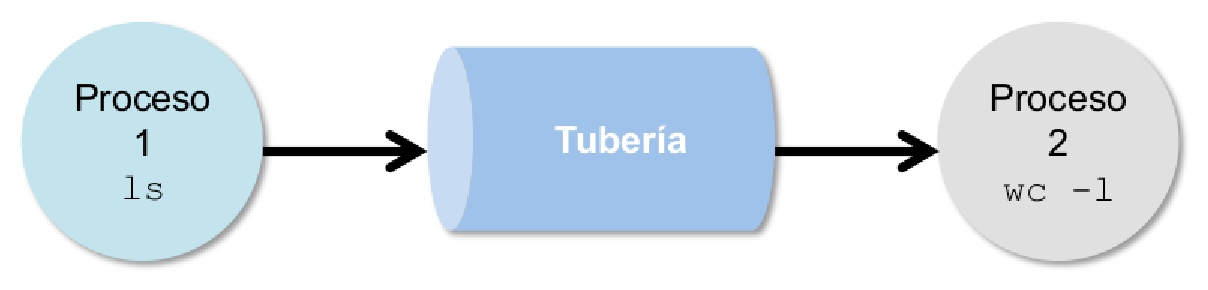
\includegraphics[scale=0.4]{figs/flujo_pipe}
\caption{Flujo de datos en una tubería.}
\label{fig:FlujoPipe}
\end{figure}


El alumno ya se familiarizó en la práctica 2 con tuberías a nivel de intérprete de órdenes. Un ejemplo sencillo es el siguiente:

\begin{lyxcode}
\texttt{ls | wc -l}
\end{lyxcode}

Para ejecutar la orden anterior, el \textit{shell} crea dos procesos (con el servicio POSIX \texttt{fork()}). Cada uno de ellos ejecuta, mediante un servicio POSIX de la familia \texttt{exec()}, las órdenes \texttt{ls} y \texttt{wc -l}, respectivamente (los servicios POSIX \texttt{fork()} y \texttt{exec()} ya se han descrito en la sección \ref{sec:Procesos}).

Las tuberías o \textit{pipes}, propiamente dichos, son un mecanismo de comunicación sin nombre. Por esta razón, sólo pueden usarse por el proceso que lo cree y sus procesos hijos, que heredan el \textit{pipe}\footnote{Existe otra variación de tuberías, las tuberías FIFO o tuberías con nombre, utilizadas para comunicar y sincronizar varios procesos independientes. Este tipo de tuberías no será objeto de estudio en la asignatura de Sistemas Operativos.}. 


%Como puede observarse en la figura anterior, el proceso que escribe, \texttt{ls}, tiene su salida estándar (con descriptor de archivo 1) unida al extremo de escritura de la tubería mientras que el proceso que lee, \texttt{wc -l}, tiene su entrada estándar (con descriptor de archivo 0) unida al extremo de lectura de la tubería. El shell es el responsable de establecer y gestionar la tubería para que el mecanismo funcione de esa forma (queda ver cómo a continuación de forma breve). Algunas de sus características son las siguientes:


Desde el punto de vista de la implementación, una tubería es un \textit{byte stream}, es decir, se pueden leer bloques de datos independiente del tamaño de los bloques escritos por el otro extremo de la tubería y el flujo es secuencial (los bytes se leen de la tubería en el mismo orden en que fueron escritos). Las tuberías normalmente se implementan como un buffer (generalmente circular) cuyo tamaño depende del sistema operativo (tIpicamente, de 4 KB). Se dice que es un \textit{pseudoarchivo} mantenido en memoria por el sistema operativo.
%No es posible acceder aleatoriamente a los datos en un tubo usando lseek ().

La lectura y escritura de y en la tubería, respectivamente, se realiza con los mismos servicios POSIX que para leer/escribir de/en archivos. Estas APIs se verán más adelante en esta sección.


\subsubsection{Servicio POSIX \texttt{pipe()}}\label{sec:ServiciosPipe}

Un \textit{pipe} se identifica mediante dos descriptores de archivo en UNIX; uno para leer de la tubería y otro para escribir en ella. Cada proceso debe cerrar los descriptores que no utilice. El servicio POSIX que permite crear una tubería es \texttt{pipe()} cuya sintaxis es la siguiente:

\begin{lyxcode}
int~pipe(int~filedes[2]);
\end{lyxcode}

\textbf{Parámetros}

\begin{description}

\item [{filedes[ ]}] Si \texttt{pipe()} se realiza correctamente, la llamada devuelve en este array los descriptores de dos archivos abiertos que se utilizan como identificadores. \texttt{filedes[0]} se utiliza para leer de la tubería y \texttt{filedes[1]} para escribir en ella (véase Figura \ref{fig:creacionPipe}).

\end{description}

\begin{figure}[ht!]
\centering
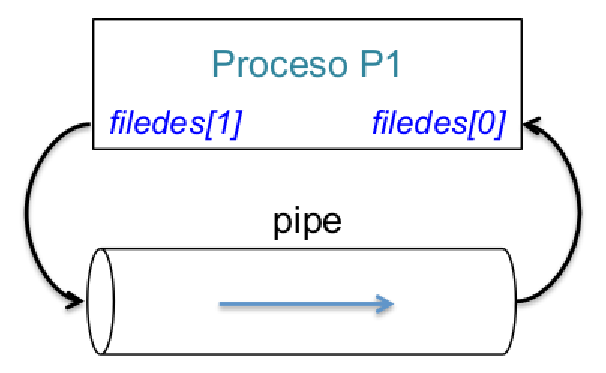
\includegraphics[scale=0.5]{figs/creacion_pipe}
\caption{Creación de una tubería con \texttt{pipe()}.}
\label{fig:creacionPipe}
\end{figure}


El servicio POSIX \texttt{pipe()} devuelve \texttt{0} en caso de éxito y \texttt{-1} si hubo algún error.\\

\subsubsection{Servicio POSIX \texttt{close()}}

El servicio POSIX \texttt{close()} permite cerrar el descriptor de archivo asociado a una tubería. 

Cerrar los descriptores de archivo de una tubería no utilizados por los procesos que manejen el \textit{pipe} es fundamental para su correcto uso, principalmente por las siguientes razones: 
\begin{itemize}
\item El conjunto de descriptores de archivo abiertos es limitado. Si un descriptor no se usa, debe cerrarse para poder ser utilizado, si fuera necesario, por otro proceso.
\item Si un proceso lee de la tubería, debe cerrar el descriptor de archivo para la escritura de tal modo que, cuando el otro proceso completa la escritura y cierra el descriptor asociado, el proceso lector detectará fin de archivo, tras haber leído los datos restantes en la tubería. En caso contrario, el proceso lector, al no cerrar el descriptor de escritura, no detectaría fin de archivo después de leer todos los datos de la tubería y una lectura posterior bloquearía la espera de datos dado que para el núcleo hay aún un descriptor de archivo de escritura abierto para la tubería. %Por otro lado, si un proceso escribe en la tubería, cierra su descriptor de lectura para la tubería. 
\item Si un proceso intenta escribir en una tubería para la que no hay ningún descriptor de archivo de lectura abierto, el núcleo del sistema operativo envía una señal \texttt{SIGPIPE} al proceso de escritura. Por defecto, esta señal mata al proceso que la recibe pero éste puede también establecer la captura o ignorar esta señal, en cuyo caso la escritura en la tubería falla con el error EPIPE (tubería rota). Recibir esa señal u obtener ese error es una indicación útil sobre el estado de la tubería por lo que se deben cerrar los descriptores de lectura no utilizados para la tubería.
Además, si el proceso de escritura no cierra el extremo de lectura de la tubería, entonces, incluso después de que el otro proceso cierre el extremo de lectura de la tubería, el proceso de escritura seguirá siendo capaz de escribir en la tubería. Eventualmente, el proceso de escritura llenaría la tubería y un intento adicional de escritura bloquearía indefinidamente al proceso.

\item Sólo después de que todos los descriptores de archivo en todos los procesos que utilicen la tubería se cierren, la tubería se destruye y sus recursos se liberan para su posible reutilización por otros procesos. En este punto, todos los datos no leídos de la tubería se pierden.
\end{itemize}


\begin{lyxcode}
int~close(int~fd);\\
\end{lyxcode}

\textbf{Parámetros}

\begin{description}
\item [{fd}] Indica el descriptor de archivo que se pretende cerrar.
\end{description}

El servicio POSIX \texttt{close()} devuelve \texttt{0} en caso de éxito y \texttt{-1} si hubo algún error.\\%\footnote{Una tubería se destruye cuando se cierra el último de sus descriptores asociados}\\

En la Figura \ref{fig:pipe_comunicacion} se muestra el uso de una tubería creada con \texttt{pipe()} para comunicar dos procesos. El proceso hijo, creado mediante el servicio POSIX \texttt{fork()}, hereda una copia de los descriptores de archivo de su proceso padre; entre ellos, los descriptores de archivo de la tubería creada por él (ver Figura \ref{fig:trasfork}).

\begin{figure}[htbp]
  \centering
  \fbox{
      \subfigure[Después de usar \texttt{fork()}]{
        \label{fig:trasfork}
        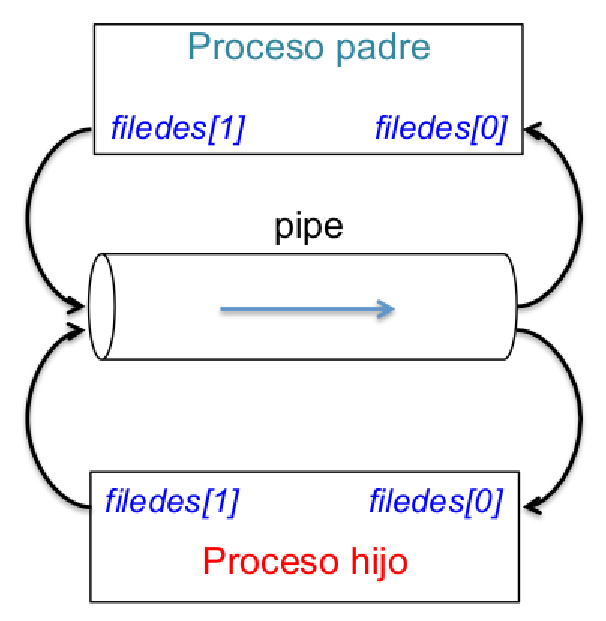
\includegraphics[scale=0.5]{figs/pipe_despues_fork}
      }
  
  
      \subfigure[Después de cerrar los descriptores no usados]{
         \label{fig:cierreDescriptores}
         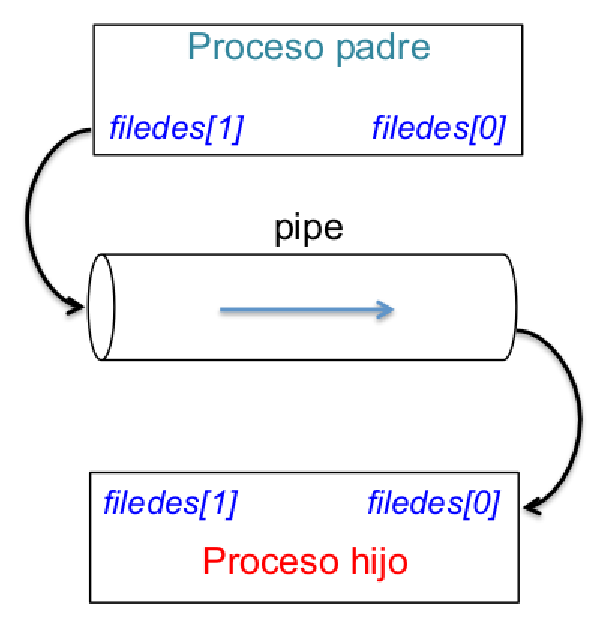
\includegraphics[scale=0.52]{figs/cierre_descr_no_usados}
      }
  }
  \caption{Creación de un \textit{pipe} para transferir datos de un proceso padre a un proceso hijo.}
  \label{fig:pipe_comunicacion}
\end{figure}

Como puede observarse en la Figura \ref{fig:pipe_comunicacion}, inmediatamente después de usar \texttt{fork()}, el proceso padre cierra su descriptor de lectura de la tubería y el hijo cierra su descriptor de escritura en la tubería. En este caso, la comunicación consiste en que el padre envía datos al hijo (ver Figura \ref{fig:cierreDescriptores}).


\subsubsection{Servicio POSIX \texttt{read()}}

El servicio POSIX \texttt{read()} se utiliza para leer datos de una tubería en el orden en el que fueron introducidos\footnote{El servicio POSIX \texttt{read()} se utiliza también en UNIX para leer datos de un archivo.}.

\begin{lyxcode}
int~read(int~fd,~char *buffer,~int~n);\\
\end{lyxcode}

\textbf{Parámetros}

\begin{description}
\item [{fd}] Descriptor de archivo utilizado para leer datos de la tubería.
\item [{buffer}] Buffer de memoria donde se pretende almacenar los datos leídos del \textit{pipe} (la operación actualiza el puntero de lectura en la tubería).
\item [{n}] Número de bytes que se desean leer de la tubería.
\end{description}

El servicio POSIX \texttt{read()} devuelve el número de bytes leídos en caso de éxito y \texttt{-1} si hubo algún error.

El proceso que lee de una tubería puede leer bloques de cualquier tamaño, independientemente del tamaño de los bloques escritos por el proceso de escritura en la tubería. 
%Puede haber múltiples procesos lectores.

A continuación, brevemente, se detalla la semántica de la operación de lectura de una tubería:
\begin{itemize}

\item Si el tamaño de la tubería es T y se desea leer de ella un número de bytes mayor, la operación devolverá T bytes. En caso contrario, la operación devuelve n bytes. En ambos escenarios, se eliminan los datos leídos de la tubería.
\item Si se cierra el extremo final de escritura de la tubería y no hay procesos escritores, la operación de lectura de la tubería devolverá 0 bytes (final de archivo) una vez que haya leído los datos restantes de la tubería, pero no bloquea al proceso lector.
\item La operación se lleva a cabo de forma \textbf{atómica}, es decir, si varios procesos intentan leer simultáneamente en una tubería, sólo uno de ellos podrá hacerlo y el resto de procesos se bloqueará hasta que finalice esa lectura. La atomicidad de esta operación se garantiza cuando el número de datos que se intentan leer es menor que el tamaño de la tubería.
\item Si la tubería está vacía, la invocación a \texttt{read()} bloqueará al proceso que realiza la lectura hasta que otro proceso escriba datos en la tubería\footnote{Se puede evitar el bloqueo usando modo de lectura no bloqueante con el servicio POSIX \texttt{fcntl()}.}. 
\end{itemize}


\subsubsection{Servicio POSIX \texttt{write()}}

El servicio POSIX \texttt{write()} se utiliza para escribir datos de forma ordenada en una tubería\footnote{El servicio POSIX \texttt{write()} también se utiliza en UNIX para escribir datos en un archivo.}.

\begin{lyxcode}
int~write(int~fd,~char *buffer,~int~n);\\
\end{lyxcode}

\textbf{Parámetros}

\begin{description}
\item [{fd}] Descriptor de archivo que se utiliza para escribir datos en la tubería.
\item [{buffer}] Buffer de memoria donde se localizan los datos que se van a escribir en la tubería (la operación actualiza el puntero de escritura de la tubería).
\item [{n}] Número de bytes a escribir en la tubería.
\end{description}

El servicio POSIX \texttt{write()} devuelve el número de bytes escritos en caso de éxito y \texttt{-1} si hubo algún error.

A continuación, brevemente, se detalla la semántica de la operación de escritura en una tubería:

\begin{itemize}

\item Si no hay ningún proceso con la tubería abierta para lectura, el sistema operativo envía la señal \texttt{SIGPIPE} al proceso que pretende escribir. El proceso recibe la señal \texttt{SIGPIPE} y la operación de escritura (\texttt{write()}) devolverá un error.
\item La operación se lleva a cabo de forma \textbf{atómica}, es decir, si varios procesos intentan escribir simultáneamente en una tubería, sólo uno de ellos podrá hacerlo y el resto de procesos se bloqueará hasta que finalice esa escritura. La atomicidad en la escritura se garantiza, al igual que para la lectura, cuando el número de datos que se intentan escribir es menor que el tamaño de la tubería.
\item Si la tubería está llena o se llena durante la escritura actual, esta operación bloqueará al proceso escritor hasta que se pueda completar la operación.
\end{itemize}


\subsubsection{Servicios POSIX para redirecciones: \texttt{dup()} y  \texttt{dup2()}} 

%44.4. Contar el porqué de su uso general y cuando se usa como en el ejemplo de la tubería para conectar ls y un filtro
Las redirecciones ya se vieron en la práctica 2 a nivel del intérprete de órdenes y qué operaciones y tablas están involucradas en espacio de usuario y espacio de núcleo. Del mismo modo, este concepto es clave en el caso de uso de órdenes comunicadas con tuberías como el ejemplo \texttt{ls~|~wc -l}. En este caso, se trata de dos redirecciones; en primer lugar, la salida estándar de la orden \texttt{ls} debe ser redirigida a la entrada de la tubería (extremo de escritura) y la entrada de la orden \texttt{wc -l}  debe ser redirigida a la salida de la tubería (extremo de lectura). Para realizar estas dos redirecciones deben usarse los servicios POSIX \texttt{dup()} o \texttt{dup2()}. Ambos, se utilizan para duplicar un descriptor de archivo. Los prototipos de estas dos funciones son los siguientes:

\begin{lyxcode}
int~dup(int~fd);\\
int~dup2(int~fd, int~new\_fd);\\
\end{lyxcode}

\textbf{Parámetros}

\begin{description}
\item [{fd}] Descriptor de archivo cuya entrada en la tabla de descriptores de archivo (TDA) va a ser duplicada en otra (en concreto, en la entrada más baja libre).
\item [{new\_fd}] Descriptor de archivo cerrado inicialmente por \texttt{dup2()} para, posteriormente, copiar en su entrada en la TDA la del primer parámetro, \texttt{fd}.
\end{description}


Los servicios POSIX \texttt{dup} y \texttt{dup2} devuelven el nuevo descriptor de archivo en caso de éxito y \texttt{-1} si hubo algún error.

El siguiente ejemplo muestra cómo puede usarse \texttt{dup()} o \texttt{dup2()} para redigir la salida estándar de un proceso.\\
\\
\noindent\texttt{/* uso de dup() */}\\
\texttt{int fd[2];}\\
\texttt{pipe(fd);}\\
\\
\texttt{/* código adicional */}\\
\\
\texttt{close(STDOUT\_FILENO);}\\
\texttt{dup(fd[1])}\\

Sin embargo, piense qué puede suceder si, con el fragmento de código anterior, utilizando \texttt{dup()} en vez de \texttt{dup2()},  la entrada estándar (\texttt{STDIN\_FILENO}), con descriptor de archivo 0, ha sido cerrada antes de invocar a \texttt{dup()}. Para evitar errores, es conveniente usar \texttt{dup2()} como se muestra a continuación:\\
\\
\noindent\texttt{/* uso de dup2() */}\\
\texttt{int fd[2];}\\
\texttt{pipe(fd);}\\
\\
\texttt{/* código adicional */}\\
\\
\texttt{dup2(fd[1], STDOUT\_FILENO)}\\

A continuación, como ejemplo de manejo de los servicios POSIX de pipes, se muestra el código que implementa la ejecución de la tubería \texttt{ls~|~wc}\footnote{En él, por brevedad, se han obviado las comprobaciones de error de la mayoría de servicios POSIX utilizados (\texttt{pipe()}, \texttt{close()}, \texttt{wait()}, etc.).}. Además, en la Figura \ref{fig:EjemploTuberia} se muestran las principales operaciones realizadas en la implementación del uso de la tubería por las dos órdenes implicadas en este ejemplo.

\lstinputlisting[language={[ANSI]C},basicstyle=\footnotesize\ttfamily,lineskip=-0.9mm,
    tabsize=2, frame=lines, inputencoding=latin1,,
    extendedchars=true]{ejercicio2/ejemplo_tuberia.c}

\begin{figure}[ht!]
\centering
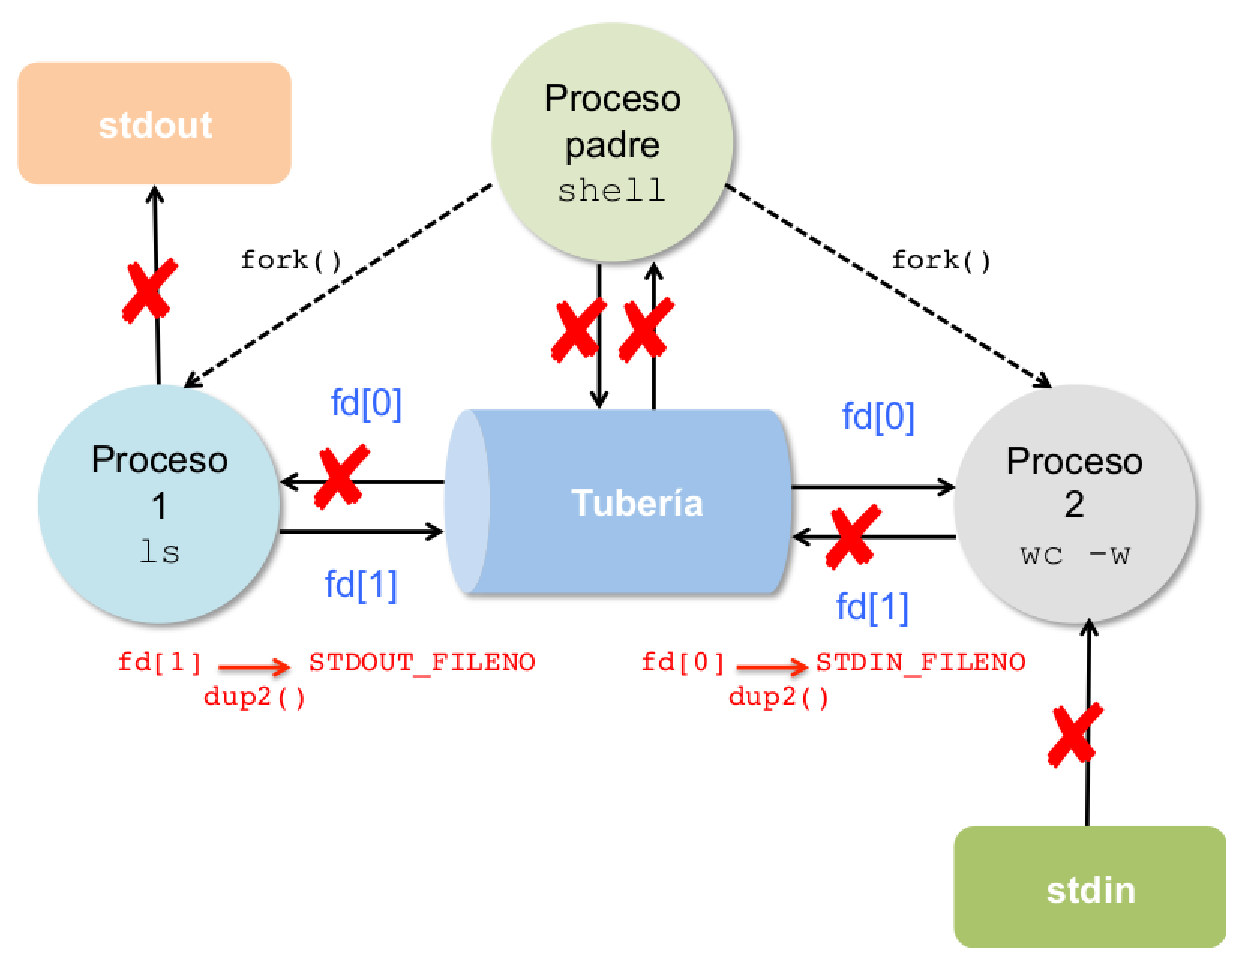
\includegraphics[scale=0.45]{figs/ejemplo_tuberias}
\caption{Esquema sobre la implementación de la orden \texttt{ls~|~wc -l.}}
\label{fig:EjemploTuberia}
\end{figure}

Compruebe el resultado de este programa. 
%¿Y el siguiente código, qué hace?

%\medskip
%\lstinputlisting[language={[ANSI]C},basicstyle=\footnotesize\ttfamily,lineskip=-0.9mm,
%    tabsize=2, frame=lines, inputencoding=latin1,,
%    extendedchars=true]{ejercicio2/ejemplo2_tuberia.c}





\section{Intérprete de órdenes}

El intérprete de órdenes es la puerta de entrada tradicional a UNIX.
Comprender su funcionamiento interno ayuda
a comprender muchos de los conceptos básicos de interacción con el
sistema operativo, diferenciar bien los espacios de usuario y de sistema, así como algunos mecanismos de comunicación entre procesos.


\subsection{Ciclo de ejecución del intérprete de órdenes}\label{sub:CicloShell}

Conviene conocer la secuencia de acciones que realiza el intérprete
de órdenes, que consiste básicamente en los siguientes pasos:
\begin{enumerate}
\item {\em Imprimir del prompt}. El intérprete se encuentra a la espera de que el
usuario introduzca una orden.
\item {\em Procesar la orden (\textit{parser})}. Se realizan un conjunto de transformaciones sobre la orden del usuario. Por ejemplo,
si el usuario ha introducido \texttt{cat practica1.c}, el intérprete transforma la cadena anterior en una estructura que pueda ser manejada más fácilmente en su ejecución (como ya veremos, consiste, esencialmente, en la transformación de la cadena en un array de vectores a las cadenas ``\texttt{cat}'' y ``\texttt{practica1.c}'').

\item {\em Interpretar la orden}. Antes de ejecutar la orden, se realizan un conjunto de funcionalidades como sustituir variables del \textit{shell} por sus valores, generar nombres de archivos a partir de metacaracteres que aparezcan en la orden, o manejar las redirecciones y tuberías. Por ejemplo, si el usuario ha introducido la orden \texttt{ls *.pdf}, y en el
directorio de trabajo hay dos archivos, \texttt{examen.pdf} y \texttt{solucion.pdf},
el intérprete transforma \texttt{ls *.pdf} en \texttt{ls examen.pdf solucion.pdf}. Este es un ejemplo de generación de nombres de archivo a partir del metacarácter '*' que realiza el \textit{shell}.

\item {\em Ejecutar la orden}. En función de cuál sea el tipo de orden introducido, el proceso de ejecución
de la orden es  bien distinto. El \textit{shell} verifica si es una \textit{orden interna}. Si lo es, ejecuta su código, perteneciente (interno) al propio código del intérprete de órdenes. En caso contrario, se trata de un programa ejecutable de UNIX (independiente del \textit{shell}); si es una \textit{orden externa}, el intérprete busca su imagen binaria (ejecutable) para solicitar su ejecución al Sistema Operativo\footnote{La petición de ejecución se realiza mediante el uso conjunto de los servicios POSIX \texttt{fork()} y \texttt{exec()}, respectivamente.}.

\end{enumerate}

\begin{figure}[ht!]
\begin{centering}
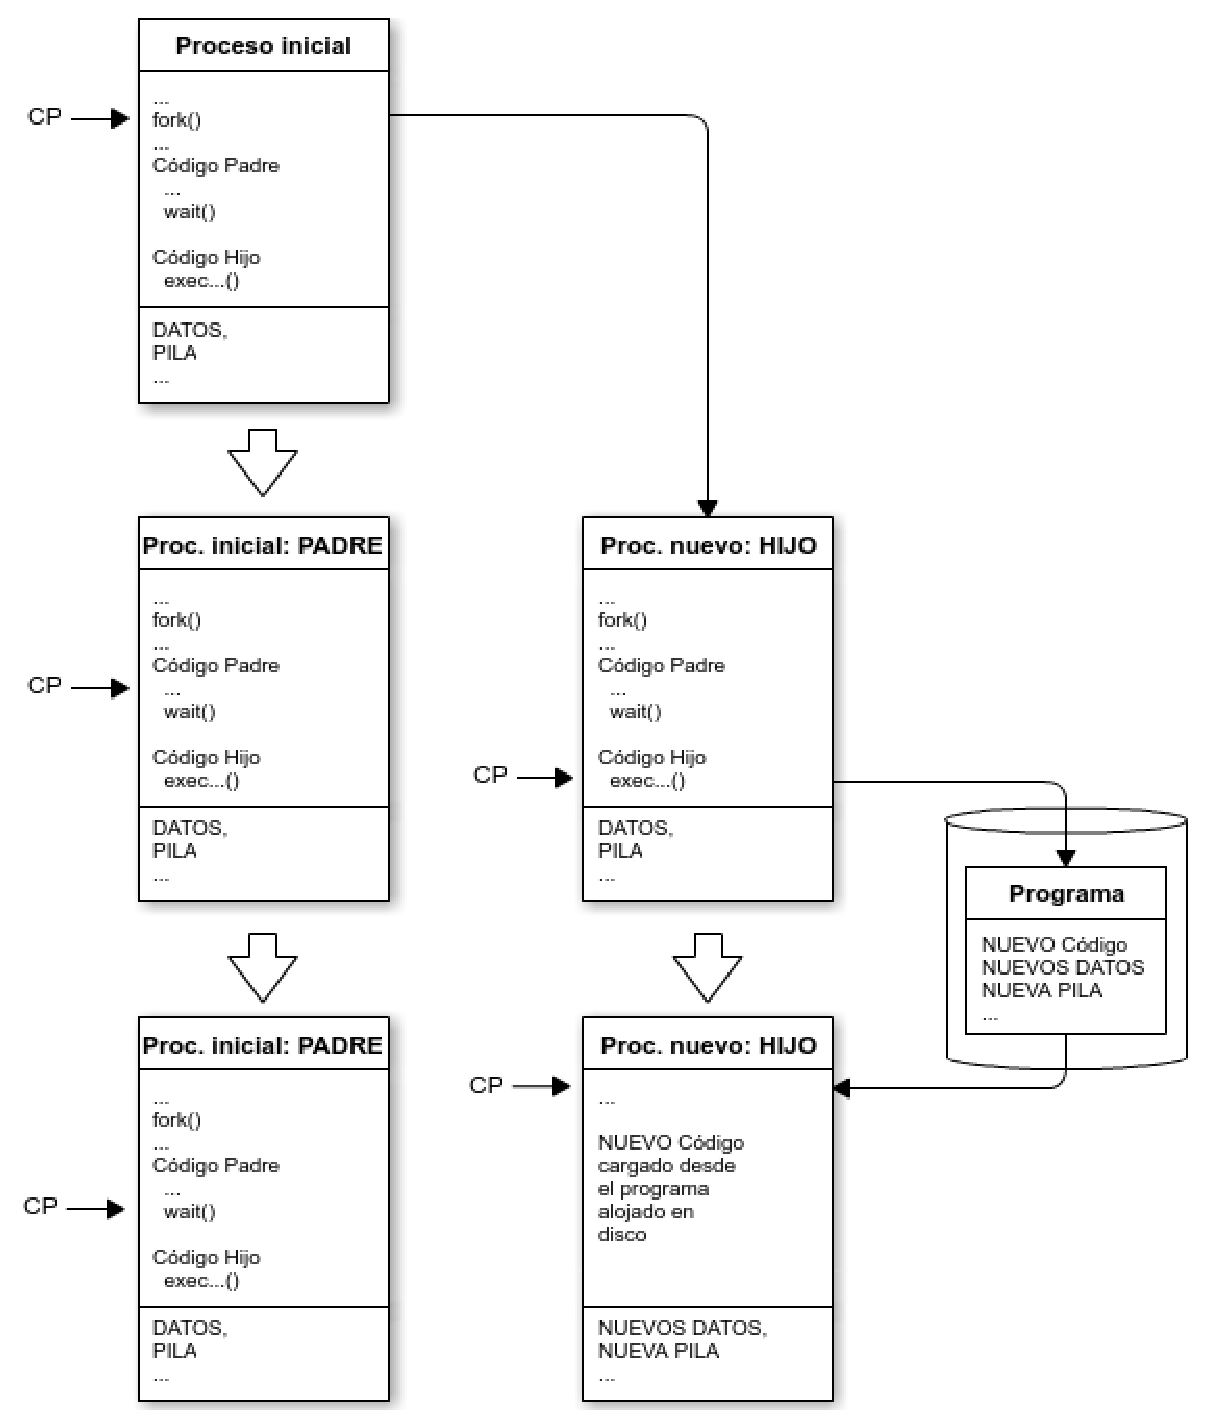
\includegraphics[scale=0.52]{figs/ejecucionShell1}
\par\end{centering}

\caption{\label{cap:Ejecucion-de-una}Ejecución de una orden externa
dentro de un intérprete de órdenes.}

\end{figure}


\section{Ejercicio}

Como aplicación de los servicios POSIX de gestión de procesos descritos, el alumno debe completar el desarrollo, en lenguaje C y sobre sistema
operativo Linux, de una aplicación a la que denominaremos \emph{minishell}. Esta aplicación se comportará como una versión reducida de un
intérprete de órdenes de UNIX (en concreto, de \textit{bash}).

Como cualquier proceso en UNIX, \textit{minishell} utilizará por defecto la entrada estándar -teclado- (cuyo descriptor de archivo es 0) para leer las líneas de órdenes a interpretar y ejecutarlas, y la salida estándar -pantalla- (cuyo
descriptor de archivo es 1) para presentar el resultado de las órdenes
ejecutadas. Y, para notificar los errores que se puedan producir,
usará por defecto la salida estándar de errores -pantalla- (cuyo descriptor de archivo es 2).
%Si ocurriera algún error al invocar un servicio POSIX, se notificará mediante la función de biblioteca \texttt{perror()}.

Las tareas a realizar en el desarrollo de la \textit{minishell} son las siguientes:


\begin{enumerate}
%\newpage
\item Implementar las funcionalidades siguientes en \textit{minishell}:

\begin{itemize}

\item Ejecución de órdenes simples externas en primer plano (por ejemplo, \texttt{ls -l},
\texttt{who}, etc.). Para ejecutar una orden externa en primer plano debe crearse
un proceso \textit{minishell} hijo (veáse información con: \texttt{man 2 fork}) que ejecute mediante el servicio
\texttt{exec()} (véase información con: \texttt{man 2 execvp}) el archivo binario asociado a la orden.
Mientras tanto, el proceso padre (\textit{minishell} padre) debe esperar a
la finalización del proceso hijo (véase información con: \texttt{man 2 wait}). Al final de la orden \textbf{no} existe el símbolo \texttt{'\&'}. 

\item Ejecución de la orden interna \texttt{exit}. Cuando la aplicación \textit{minishell} reciba esta orden, finalizará su ejecución. 
\item Ejecución de órdenes internas.  Sólo se podrán ejecutar como órdenes  internas, además de \texttt{exit}, \texttt{umask}, \texttt{cd}, \texttt{pwd} y  \texttt{declare}\footnote{La implementación de estas  órdenes, como se reiterará más adelante, se proporciona al alumno en el archivo  objeto  \texttt{internas.o}.}


\item Ejecución de órdenes en \emph{background} (usando el carácter \texttt{'\&'}
al final de las órdenes). Cuando la \textit{minishell} detecte este símbolo al final de una orden, no debe esperar a la terminación del proceso hijo creado para ejecutarla sino que, inmediatamente, imprimirá el \emph{prompt} para aceptar una nueva orden.


\item Ejecución de secuencias de órdenes separadas por el símbolo \texttt{';'} (\textbf{como mínimo}, secuencias de órdenes externas). 
\item Ejecución de órdenes con redirecciones de entrada (\texttt{<}) y salida (\texttt{>}).
\item Ejecución de órdenes externas compuestas (separadas mediante tuberías).

\end{itemize}


\item Crear un archivo \textit{Makefile} que permita la compilación automatizada de la aplicación. %\textit{Obligatorio}.

\item Realizar las pruebas adecuadas de \textit{minishell}. %\textit{Obligatorio}. 

\end{enumerate}

% falta ver si al final se entrega libshell.a o bien -casi seguro que sí-, se da el fuente de las funciones de biblioteca para que creen ellos con una regla en el makefile


% revisar siguiente párrafo según lo anterior
Para el desarrollo de este ejercicio utilice los archivos fuente y archivos de cabecera que se proporcionan como material de apoyo con la práctica. Realice con ellos las fases que a continuación se detallan, de forma incremental y modular, siguiendo los pasos que se indican en cada una de ellas y probando poco a poco las funcionalidades que se vayan codificando.\\

\begin{bclogo}[couleur = mycolor,arrondi =0.1, logo = \bcinfo, ombre = false]{\small{\textbf{Diagrama de la estructura de \textit{minishell}}}}
\small{En el Anexo A se adjunta un diagrama de la estructura detallada de la aplicación \textit{minishell}. El esquema muestra los diferentes archivos, la relación existente entre ellos y las funciones que incluyen distinguiendo si están ya implementadas o no. Se recomienda al alumno tenerlo a mano en todo momento para tener una visión global de toda la aplicación y  poder ubicar cada función en el conjunto.}
\end{bclogo}

% aquí indicar: En el anexo A se proporciona un diagrama que muestra la estructura detallada de la minishell. En él, se representan con rectángulos los módulos que forman parte de la aplicación y la relación entre ellos y que a continuación se detallan: 1) los archivos fuente que forman parte de la minishell, 2) los archivos de cabecera necesarios para el preprocesado de cada uno de ellos, 3) la biblioteca proporcionada, sus archivos en código objeto y las funciones que incluyen. Los módulos cuya implementación se proporciona al alumno se representan con rectángulos en blanco mientras que los que debe completar se representan diferenciados en color verde. Asimismo, en este diagrama se representa la relación entre ellos. El alumno debería acceder en todo momento a este diagrama para ubicar cada función descrita en este ejercicio y confirmar si ya es proporcionada o debe ser implementada así como la relación con otros módulos de la aplicación.

%En cada fase se especifica su carácter \textit{Obligatoria} u \textit{Optativa}. \textit{Fase Obligatoria}: su realización es requisito imprescindible para tener apta la parte práctica %de la asignatura. Bloque \textit{Optativo}: el alumno puede optar a su desarrollo para mejorar la valoración de la práctica 3 pero no es necesaria su realización.\\
\medskip

A continuación, realice las fases que se van describiendo en las siguientes secciones para el desarrollo de \textit{minishell}.\\
\medskip

%\begin{itemize}
\subsection{FASE 1: Ciclo de ejecución de órdenes}\label{sub:Fase1Shell}

\medskip
Edite el archivo fuente denominado \textbf{minishell.c}. Complete este código definiendo la función principal (\texttt{main()}) encargada de realizar, de forma reducida, acorde exclusivamente a las funciones que  se van a incluir en esta práctica, el ciclo de ejecución de órdenes del \textit{minishell} (véase sección \ref{sub:CicloShell}). Para ello, siga el diagrama de la Figura \ref{fig:mainMinishell}. 


%incluir parte del código para variables introducidas poder modificarlar

\medskip
\lstinputlisting[language={[ANSI]C},basicstyle=\footnotesize\ttfamily,lineskip=-0.9mm,
    tabsize=2, frame=lines, inputencoding=latin1,numbers=left,
    extendedchars=true, caption=\texttt{minishell.c} incompleto]{ejercicio2/minishellincompleto.c}
    
\medskip
\begin{figure}[ht!]
\centering
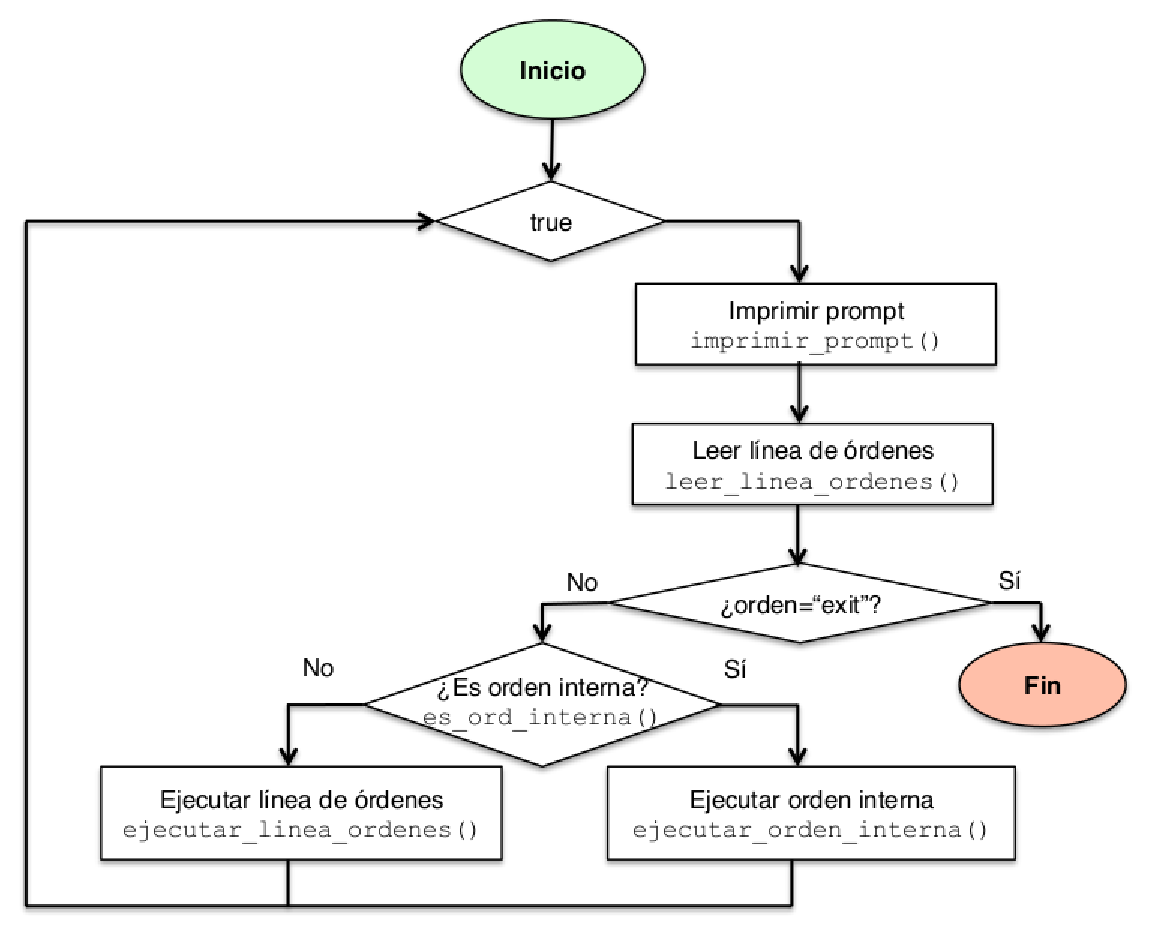
\includegraphics[scale=0.6]{figs/mainaccesibilidadtotal}
\caption{Diagrama de la función \texttt{main()} de \textit{minishell}.}
\label{fig:mainMinishell}
\end{figure}

Posponga el tratamiento de una orden externa (invocación a \texttt{ejecutar\_linea\_ordenes()} de la Figura \ref{fig:mainMinishell}) hasta la realización de la \textbf{FASE 2} de la práctica (se trata de ir resolviendo y probando poco a poco las tareas que se solicitan).

Como puede observar en la Figura \ref{fig:mainMinishell}, para implementar la función \texttt{main()} se utilizan sendas funciones: \texttt{imprimir\_prompt()}, \texttt{leer\_linea\_ordenes()}, \texttt{es\_ord\_interna()} y \texttt{ejecutar\_ord\_in-\\terna()}. El código de estas funciones se proporciona como material de apoyo. Sólo debe invocarlas adecuadamente teniendo en cuenta en qué archivos se encuentran tanto la definición como el prototipo de cada una de ellas. A continuación, se proporciona también una descripción de estas funciones\footnote{Estas funciones se han codificado de forma sencilla para que el alumno las pueda interpretar fácilmente y vaya familiarizándose con el lenguaje C. Puede modificar y simplificar las funciones relacionadas con entrada/salida de C. La correcta adaptación de su codificación será valorada en la nota final de la práctica.}:
\vspace{0.3cm}	
% poner con una advertencia dónde localizarlas (ver Figura correspondiente en ANEXO).
\begin{itemize}

\item\texttt{\textbf{void imprimir\_prompt()}}. Imprime el prompt de la \textit{minishell}. %Esta función se encuentra en el archivo \textbf{entrada\_minishell.c}.
\vspace{0.3cm}


\item\texttt{\textbf{void leer\_linea\_ordenes(char *buf)}}. Lee la línea de órdenes de la entrada estándar y la almacena como una cadena de caracteres en \texttt{buf}. % Esta función se encuentra en el archivo \textbf{entrada\_minishell.c}.

% Analice el código de la función \textbf{leer\_linea\_ordenes()}. Utiliza la función \textbf{eliminar\_salto\_linea()} para eliminar el salto de línea (carácter \'\\n\') que existe al leer con la función fgets() la línea de órdenes, antes de almacenarla 
\vspace{0.3cm}

\item \texttt{\textbf{int es\_ord\_interna(const char *buf)}}. Devuelve si la orden que se pasa como argumento es interna (valor 1) o externa (valor 0). Las \textbf{únicas} órdenes internas implementadas son: \texttt{cd}, \texttt{pwd}, \texttt{declare} y \texttt{umask}.%\footnote{La codificación proporcionada al alumno de las 4 órdenes internas es parcial. La correcta programación de funcionalidades añadidas en alguna de ellas será valorada en la nota final de la práctica.}. 
\vspace{0.3cm}
\item \texttt{ejecutar\_ord\_interna(const char *buf)}. Si la orden que se pasa como argumento es interna, la función ejecuta la orden.\\%y 
Las dos primeras funciones se encuentran en el archivo \texttt{entrada\_minishell.c} proporcionado como material de apoyo. Las dos últimas, relacionadas con órdenes internas, se proporcionan en el archivo en código objeto \texttt{internas.o}.

\end{itemize}

Consulte el diagrama de la aplicación \textit{minishell} (Apéndice \ref{sec:Aped.A}) para comprobar los archivos que se proporcionan como material de apoyo. De momento, se recomienda no crear la biblioteca estática \texttt{libshell.a}; ya lo hará más tarde. Para probar esta fase sólo precisa usar los archivos fuente y de cabecera requeridos así como el archivo  \texttt{internas.o} en la compilación.
%Adicionalmente, se proporcionan como material de apoyo los archivos \texttt{entrada\_mini-\\shell.h} (archivos de cabecera de \texttt{entrada\_minishell.c}), \texttt{internas.h}  y  \texttt{parser.h}, archivos de cabecera asociados a los archivos objeto, \texttt{internas.o} y \texttt{parser.o}, incluidos en \texttt{libshell.a}, biblioteca también proporcionada así como el archivo \texttt{libmemoria.c} y su archivo de cabecera \texttt{libmemoria.h} (véase \ref{sec:Aped.A}).\\

\begin{bclogo}[couleur = mycolor,arrondi =0.1, logo = \bcpanchant, ombre = false]{\small{\textbf{Desarrollo incremental y pruebas}}}
\small{Se recomienda probar de forma incremental las diferentes funcionalidades programadas en todas las fases. Antes de entregar la práctica, realice la validación con las pruebas adecuadas.}
\end{bclogo}

\medskip
\subsection{FASE 2: Ejecución de órdenes externas simples en primer plano}\label{sub:EjecOrdExtPP}

\medskip
Una vez realizadas las pruebas de la ejecución de órdenes internas, realice en esta fase la implementación de órdenes externas simples y en primer plano como las que a continuación se muestran en sendos ejemplos:\\\\
\indent\texttt{minishell$>$ cut -f5 -d: /etc/passwd}\\
\indent\texttt{minishell$>$ sleep 30}\\\\
Sin embargo, una línea de órdenes como la siguiente es una orden compuesta, es decir, formada por varias órdenes comunicadas mediante tuberías, y ejecutada en \textit{background}. De la implementación de órdenes compuestas no debe preocuparse ahora:\\\\
\indent\texttt{minishell$>$ cut -f5 -d: /etc/passwd | sort > usuarios.txt \&}\\
%Como puede observarse en el ejemplo anterior, la línea de órdenes consta de dos órdenes que se comunican mediante tuberías. Además, se almacena el resultado de la ejecución de la última orden en un archivo.\\

Para realizar la tarea de esta fase, edite el archivo \textbf{ejecutar.c} proporcionado como material de apoyo. Este archivo contiene, incompletas, las funciones relacionadas directamente con la ejecución de una línea de órdenes externa. Finalice la implementación del código de \texttt{ejecutar.c} que se muestra a continuación. 

% código
\medskip
\lstinputlisting[language={[ANSI]C},basicstyle=\footnotesize\ttfamily,lineskip=-0.9mm,
    tabsize=2, frame=lines, inputencoding=latin1,,
    extendedchars=true,  caption=\texttt{ejecutar.c} incompleto]{ejercicio2/ejecutarincompleto.c}

\begin{itemize}
% completar código y hacer ejecutar.c. Paso 3: solucionar espera del padre foreground y backgroun bien hecho.
% paso 4: optativo -> separado por ;

\item \texttt{\textbf{void ejecutar\_linea\_ordenes(const char *orden)}}. Esta función se encarga de ejecutar una orden externa introducida por el usuario. Como ya se ha indicado, \textbf{sólo debe implementar en esta fase la ejecución de órdenes externas simples}. Para ello, la función invoca a \texttt{ejecutar\_orden()}, función cuya descripción se proporciona más adelante.

Tras la llamada a \texttt{ejecutar\_orden()}, \texttt{ejecutar\_linea\_ordenes()} debe comprobar la existencia o no del símbolo de \textit{background} al final de la orden,  información que es devuelta por \texttt{ejecutar\_orden()}. En función de este chequeo, \texttt{ejecutar\_linea\_ordenes()} proporcionará el siguiente tratamiento:
\begin{itemize}
\item \textbf{Si no existe el símbolo '\&'}. Se trata de una ejecución en primer plano (\textit{foreground}). El proceso padre (\textit{minishell} padre) \textbf{debe esperar} (invocando al servicio POSIX adecuado) a que el proceso hijo (\textit{minishell} hija) finalice su ejecución. Cuando esto ocurra, el proceso \textit{minishell} padre podrá realizar otra iteración del ciclo de la función \texttt{main()}. Por lo tanto, imprimirá el \textit{prompt} y volverá a leer y ejecutar otra posible orden introducida por el usuario.
\item \textbf{Si la orden termina con '\&'}. Se trata de una ejecución en segundo plano (\textit{background}). El proceso \textit{minishell} padre simplemente no debe esperar la finalización del proceso \textit{minishell} hijo y podrá volver a ejecutar \textbf{inmediatamente} otra iteración del bucle de la función \texttt{main()}. Esto significa que el proceso  \textit{minishell} padre y el proceso \textit{minishell} hijo podrán ejecutar concurrentemente órdenes. 
\end{itemize}

\item \texttt{\textbf{void ejecutar\_orden(const char *orden, int *background)}}. Función que crea un proceso \textit{minishell} hijo (invocando al servicio POSIX adecuado) para ejecutar la orden externa pasada como parámetro (\texttt{orden}). \textbf{La función devuelve en} \texttt{\textbf{background}} \textbf{el valor 1 si hay un símbolo de \textit{background} ('\&') al final de la orden}, o 0 en caso contrario.
% usar otro cuadradito
Como puede observar en el código proporcionado previamente, la función \texttt{ejecutar\_orden()}  primero invoca a la función \texttt{parser\_orden()} cuya descripción y prototipo se detallan más adelante. Esta última función es responsable de convertir la cadena \texttt{orden}, que almacena la orden externa introducida por el usuario, en una estructura que facilite su ejecución con el servicio POSIX correspondiente. La función \texttt{parser\_orden()} ya está implementada y se incluye en el archivo objeto \texttt{parser.o}. 

Antes de finalizar la definición de la función \texttt{ejecutar\_orden()}, deberá invocar a \texttt{free\_ar-\\gumentos()} ya que la función \texttt{parser\_orden()} crea un array dinámico que debe ser liberado para evitar lagunas de memoria. La función \texttt{free\_argumentos()}, cuyo prototipo se muestra a continuación, ya está implementada en el archivo \texttt{libmemoria.c}.\\

\texttt{\textbf{void free\_argumentos(char **argumentos)}}. Esta función libera la estructura \\\texttt{argumentos} de tipo array dinámico.
\medskip

\end{itemize}

\begin{bclogo}[couleur = mycolor,arrondi = 0.1, logo = \bclampe, ombre = false]{\small{Uso de la función \texttt{ejecutar\_linea\_ordenes()}}}
\small{La existencia de  \texttt{ejecutar\_linea\_ordenes()}, además de la función de \texttt{ejecutar\_orden()}, pretende ofrecer una  descomposición más modular y flexible de \textit{minishell} para dar así la posibilidad de ampliar más adelante en ella la funcionalidad solicitada en la Fase 7 (tratamiento de órdenes compuestas). El alumno puede obviarla y realizar sus tareas, indicadas previamente, en la propia función \texttt{ejecutar\_orden()}, u otra.}
\end{bclogo}

% junto con la de arriba en recuadro\\ %\footnote{Ciertamente, se observa que \texttt{ejecutar\_linea\_ordenes()} apenas añade funcionalidad a la proporcionada por \texttt{ejecutar\_orden()} para llevar a cabo esta fase y, por consiguiente, parece que su uso podría evitarse y, así es. Sin embargo, dado el interés pedagógico de esta práctica, se ha hecho un esfuerzo en que aquellos alumnos que lo deseen, lo utilicen para ir más allá de las tareas que se solicitan aquí y puedan extender el \textit{minishell} con más comodidad.}. El objetivo es permitir extender las responsabilidades de la función \texttt{ejecutar\_li\\nea\_ordenes()} fácilmente y sin necesidad de cambiar las interfaces de las funciones ya proporcionadas, de tal forma que puedan  tratarse y ejecutarse con ella no sólo órdenes externas simples, sino también líneas de órdenes compuestas como las descritas anteriormente (es decir, con tuberías y redirecciones).


\texttt{\textbf{parser\_orden()}}:\\

\textbf{Descripción}\\

Función que convierte la cadena que representa la orden introducida al ejecutar \textit{minishell}, en una nueva	
estructura: un array de punteros a cadenas. La finalidad es dejar preparada la orden para ser ejecutada adecuadamente con el correspondiente servicio POSIX. Más en detalle, \texttt{parser\_orden} analiza la cadena \texttt{orden} y genera la nueva estructura que consta de: a) Una cadena por cada uno de los argumentos de \texttt{orden}, eliminando los posibles blancos entre ellos (considerando también  el nombre de la orden como argumento) y, b) si encuentra redirecciones, añade dos cadenas: una con el carácter de la redirección y otra, con la ruta del archivo asociado a ella. Asimismo, si en \texttt{orden} hay un símbolo \texttt{'\&'} (\emph{background}), la función
lo elimina (no lo incluye en la estructura creada) pero devuelve un indicador de su existencia.\\

\begin{bclogo}[couleur = mycolor,arrondi = 0.1, logo = \bctakecare, ombre = false]{\small{¿Por qué es necesario eliminar el '\&'?}}
\small{Si no se elimina el símbolo '\&' en la estructura devuelta por la función \texttt{parser\_orden()} tendrá problemas para que el proceso \textit{minishell} hijo ejecute correctamente la orden correspondiente ¿Por qué?}
\end{bclogo}

La función también devuelve, en sendos parámetros, la posición en la nueva estructura de los caracteres de redirección que puedan existir, o -1 en caso de que no existan.\\ 
%tal y como se ha indicado ya previamente\footnote{Conviene además señalar que las tuberías no suponen más que un tipo de redirecciones hacia ellas, así que, de un plumazo, si el alumno es avispado en este sentido, puede programar con esta interfaz tanto el tratamiento de las redirecciones originadas por los caracteres de redirección como las tuberías.}.

\medskip
\textbf{Prototipo}
\begin{lyxcode}
char {*}{*} parser\_orden(const char {*}orden, int {*}indentrada,\\
~~~~~~~~~~~~~~~~~~~~~int {*}indsalida, int {*}background)\\
\end{lyxcode}

\medskip
\textbf{Parámetros}

\begin{description}
\item [{orden}] Contiene la orden introducida por el usuario al ejecutar \textit{minishell}. Esta orden va a ser analizada y convertida por la función en un array dinámico
de punteros a cadenas.

\item [{indentrada}] Puntero a un entero que representa el índice en el
array devuelto por la función donde se localiza un posible símbolo
de redirección de entrada en la orden. Si no existe este tipo de redirección, devuelve un puntero a -1.

\item [{indsalida}] Puntero a un entero que representa el índice en el
array devuelto por la función donde se localiza un posible símbolo
de redirección de salida en la orden. Si no existe este tipo de redirección, devuelve un puntero a -1.

\item [{background}] Puntero a un entero que representa la existencia (1),
o no (0), del símbolo de \textit{background} (\texttt{'\&'}). 
\end{description}\begin{tiny}

\end{tiny}
\medskip
\textbf{Valores retornados}

Array dinámico de punteros a cadenas descrito anteriormente.  Además,
la función devuelve en \texttt{background} la existencia (1) o no (0) del símbolo
\textit{background} eliminándolo del array devuelto, así como el índice
en el array donde se encuentra una redirección de entrada, en \texttt{indentrada},
o una redirección de salida, en \texttt{indsalida}. En ambos casos, si no existe redirección, devuelve -1 en el parámetro correspondiente.\\
%Cada una de estas cadenas representa, como ya se ha mencionado anteriormente, bien uno de los
%argumentos de la orden, bien una cadena que contiene un símbolo de redirección
%(si existe en la orden), o bien el archivo asociado a una redirección.

\medskip
\textbf{Ejemplo}: Si la orden, de tipo cadena constante, introducida por el usuario, y argumento de la función \texttt{parser\_orden()}, es la siguiente: \texttt{orden = ``ls -l >~archivo \&''} (véase Figura \ref{fig:paramparser}), los valores finales de cada parámetro son los que a continuación se detallan:\\


\begin{lyxcode}
indsalida~=~2

indentrada~=~-1

background~=~1
\end{lyxcode}

Además, la función devuelve un array (de tipo puntero a puntero a carácter) que se representa en la Figura \ref{fig:returnparser}. 


%

\begin{figure}[htbp]
  \centering
  \fbox{
      \subfigure[Ejemplo de argumento de \texttt{parser\_orden()}]{
        \label{fig:paramparser}
        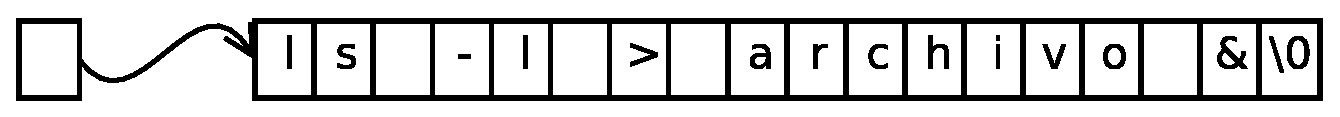
\includegraphics[scale=0.35]{figs/cadena}
      }
  
  
      \subfigure[Estructura devuelta por \texttt{parser\_orden()}]{
         \label{fig:returnparser}
         \includegraphics[scale=0.35]{figs/cadenaAnalizada}
      }
  }
  \caption{Estructuras de datos utilizadas por \texttt{parser\_orden()}.}
  \label{fig:breakgdb}
\end{figure}

% faltaría un resumen de los archivos


%\begin{center}
%
%\begin{figure*}
%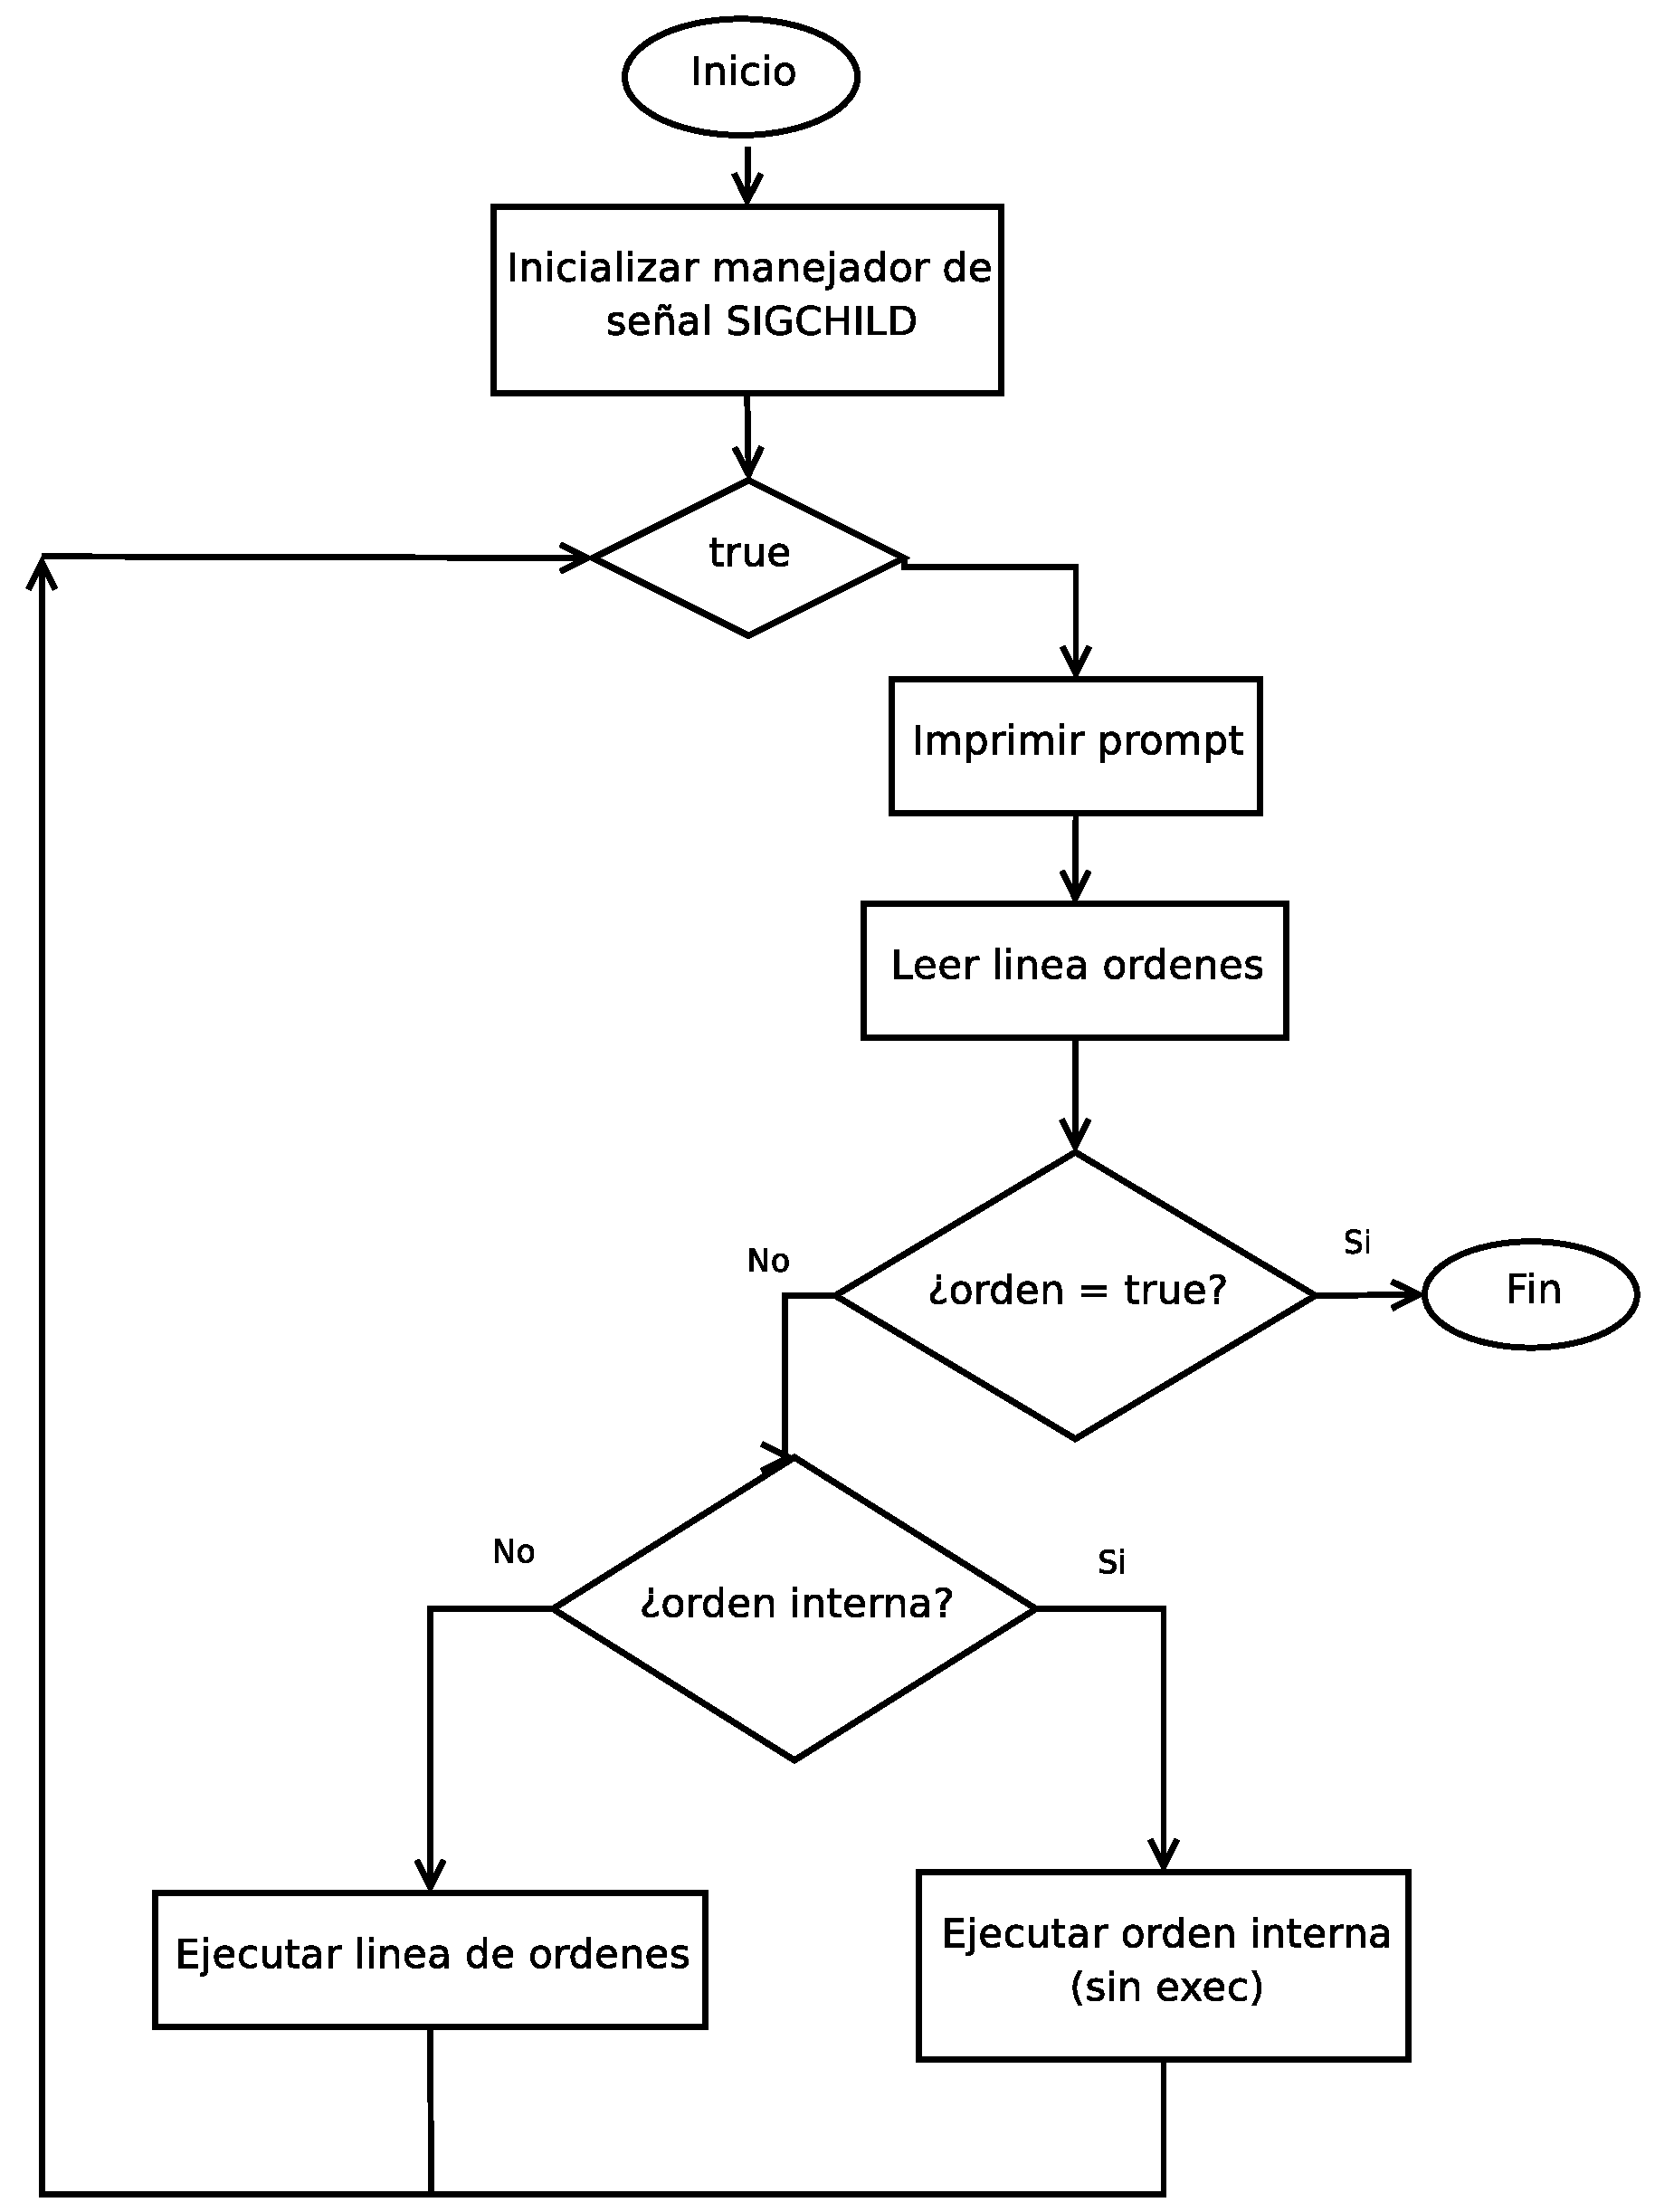
\includegraphics[scale=0.25]{minishell}

%\caption{Diagrama de flujo de la funcin \texttt{main} de \emph{minishell}.}

%\end{figure*}

%\par\end{center}
%Advertencia tipo recuadro:
%El alumno debe recordar que esta función está preparada para tratar en la Fase 6 redirecciones. En esta fase se va a utilizar únicamente para tratar órdenes externas simples sin redirecciones. Por lo tanto, las pruebas de esta fase deberán realizarse en este sentido.\\
\begin{bclogo}[couleur = mycolor,arrondi =0.1, logo = \bcinfo, ombre = false]{\small{\textbf{Versatilidad de la función \texttt{parser\_orden()}}}}
\small{\textbf{En esta fase no se tratan redirecciones} pero la interfaz así definida de \texttt{parser\_orden()} le permitirá más adelante incrementar fácilmente la funcionalidad de su \textit{minishell} programando, tras la invocación a \texttt{parser\_orden()}, y de acuerdo con los valores devueltos a través de los últimos parámetros mencionados (\texttt{indentrada} e \texttt{indsalida}), el tratamiento de las redirecciones (Fase 6, sección \ref{sub:Redirecciones}).} %Por lo tanto, realice en esta fase del desarrollo sólo pruebas de \textbf{ejecución de órdenes simples sin redirecciones}.}
\end{bclogo}

\medskip
\subsection{FASE 3: Ejecución de órdenes externas simples en segundo plano}\label{sub:EjecOrdExtBack}

\medskip
Compruebe qué sucede cuando se introduce una orden en \textit{background} con el código realizado hasta el momento. Para ello, consulte el estado de los procesos del sistema con la orden apropiada. 

Observe que el tratamiento del \textit{background} hasta esta fase puede dejar al proceso \textit{minishell} hijo en estado \textit{zombie} que, como se ha visto en en el aula, es un estado de los procesos en Linux no deseado. Razone por qué sucede esto y solucione este problema utilizando un manejador de la señal adecuada. Piense qué señal se podría utilizar para que, una vez que el proceso \textit{minishell} padre la capture, el manejador se encargue de evitar que el proceso \textit{minishell} hijo quede en estado \textit{zombie} y dónde se debería instalar el manejador. 

Una vez que tenga clara la solución al problema planteado, defina el manejador de la señal adecuadamente, de forma similar al ejemplo de manejo de la señal \texttt{SIGINT} (véase sección \ref{sub:ManejadorSennal}). Utilice para ello, ESTRICTAMENTE, la función \texttt{sigaction()},  \textbf{no }\texttt{signal()}. Asimismo, se recomienda usar la orden \texttt{man} para consultar el servicio POSIX \texttt{sigaction()}, tanto su descripción como la semántica asociada a sus parámetros.

%\textbf{\texttt{void manejar\_sigchild(char *buf)}}. Establece el manejador de la señal \texttt{SIGCHLD} para tratar correctamente el \textit{background}. Debe eliminar la task\_struct de la minishell hija que ha finalizado para evitar que quede zombie.  
%\vspace{0.3cm}

Finalmente, tras codificar esta fase, pruebe a realizar una secuencia de órdenes en \textit{background}, tal y como se muestra a continuación:\\\\
\indent\texttt{minishell$>$ sleep 12 \&}\\
\indent\texttt{minishell$>$ sleep 10 \&}\\\\
El resultado de ejecutar las órdenes previas debe ser el correcto. Una vez introducida cualquier orden en \textit{background}, el \textit{prompt} automáticamente debe volver a salir en pantalla para introducir otra orden y, además, en este escenario, \textbf{no debe haber procesos \textit{zombies} en el sistema} (no deje de probar esto último; piense con qué orden puede verificarlo).\\

\medskip
\subsection{FASE 4: Realización de \textit{Makefile}}\label{sub:CreacionMake}

\medskip
Realice el \textit{Makefile} que permita construir una nueva versión de la aplicación. 

Cree la biblioteca \texttt{libshell.a}, tal y como aparece en  el diagrama de la aplicación \textit{minishell} (Anexo A).  Para ello, defina una regla específica en el \textit{Makefile} que genere esta biblioteca estática con los archivos \texttt{internas.o} y \texttt{parser.o}, respectivamente, utilizando la herramienta \texttt{ar}\footnote{Consulte qué parámetros debe pasarle a la orden \texttt{ar} para crear la librería con el nombre de la biblioteca y el de los archivos objetos. Sugerencia: use \texttt{man}, busque en Internet o pregunte al profesor(a).}. \texttt{libshell.a} debe ser utilizada como parámetro en la invocación  a \texttt{gcc} para que los archivos objeto junto con la biblioteca se enlacen en la última fase de compilación y se genere el archivo ejecutable \textit{minishell}.

Se puntuará con 0 puntos todo archivo \textit{Makefile} que no incluya: a) definición adecuada y explícita de todas las dependencias entre los distintos archivos que componen la aplicación para generar el ejecutable \textit{minishell}, b) regla de creación de la biblioteca estática y/o, c) regla ficticia \textit{clean}.\\

\medskip
\subsection{FASE 5: Ejecución de secuencia de órdenes}\label{sub:EjecSecOrd}

\medskip
En esta fase se plantea poder ejecutar órdenes separadas por el carácter ';' (\textbf{como mínimo, secuencia de órdenes  externas})\footnote{Extender el problema a secuencia de órdenes tanto externas como internas no es complejo; ¡si le queda tiempo, inténtelo!. Se valorará en la  nota final de la práctica cualquier tarea adicional realizada.}. Cuando la aplicación \textit{minishell} detecte este símbolo, debe ejecutar de izquierda a derecha cada una de las órdenes. Resuelva este apartado declarando y definiendo su propia función e invocándola donde considere adecuado para que realice correctamente su funcionalidad. Piense que, para poder ejecutar secuencia \textbf{sólo} de órdenes externas, se trata de invocar a la función \texttt{ejecutar\_linea\_ordenes()} tantas veces como órdenes haya separadas por el carácter ';'. 


\begin{bclogo}[couleur = mycolor,arrondi =0.1, logo = \bclampe, ombre = false]{\small{\textbf{Uso  de  funciones  de manejo de cadenas de carateres de C}}}
\small{Se recomienda utilizar para esta fase funciones de manejo de cadenas de caracteres de C que pueden ser muy útiles (\texttt{strsep()}, \texttt{strtok()}, etc.).}
\end{bclogo}

\medskip
\subsection{FASE 6: Tratamiento de redirecciones}\label{sub:Redirecciones}

\medskip
En esta fase debe resolver la posibilidad de ejecutar en la aplicación \textit{minishell} órdenes externas con redirecciones de entrada o de salida. A continuación, se presenta un ejemplo con cada tipo de redirección y, finalmente, uno con ambos tipos en la misma orden:\\

\indent\texttt{minishell$>$ cut -f 5 -d : /etc/passwd > usuarios.tex}\\
\indent\texttt{minishell$>$ wc -l < /etc/passwd}\\
\indent\texttt{minishell$>$ sort  <  /etc/passwd > ordenado\_passwd \&}\\

Para resolver esta parte, edite el archivo \textbf{redirecciones.c} proporcionado como material de apoyo y que se muestra a continuación. Complete las funciones relacionadas directamente con el tratamiento de redirecciones.
% código

\medskip
\lstinputlisting[language={[ANSI]C},basicstyle=\footnotesize\ttfamily,lineskip=-0.9mm,
    tabsize=2, frame=lines, inputencoding=latin1,numbers=left,
    extendedchars=true, caption=\texttt{redirecciones.c} incompleto]{ejercicio2/redirecciones.c}
\medskip
Observe que la función \texttt{parser\_orden()} que se le ha proporcionado, descrita en la Fase 2 (sección \ref{sub:EjecOrdExtPP}), devuelve en el parámetro \texttt{indice\_entrada} la posición en la estructura \texttt{args} donde existe un  \texttt{'<'} -redirección de entrada-, o -1 en caso contrario. Del mismo modo, en el parámetro \texttt{indice\_salida} para el símbolo \texttt{'>'} -redirección de salida-. Piense qué debe hacer el código del proceso \textit{minishell} padre y del proceso \textit{minishell}  hijo, respectivamente, y retome la codificación de la función \texttt{ejecutar\_orden()} para incluir el tratamiento de ambos tipos de redirecciones. Para ello, utilice también las funciones previamente implementadas en \texttt{redirecciones.c}. 

\begin{itemize}
% completar código y hacer ejecutar.c. Paso 3: solucionar espera del padre foreground y backgroun bien hecho.
% paso 4: optativo -> separado por ;

\item \texttt{\textbf{void redirec\_entrada(char **args, int indice\_entrada, int *entrada)}}. Esta función abre convenientemente el archivo que acompaña a la redirección de entrada, localizado en \texttt{args[indice\_entrada+1]} (véase la Figura \ref{fig:returnparser})), y devuelve en el parámetro \texttt{entrada} su descriptor del archivo. % Avisar que debe desaparecer tanto el < como el archivo asociado de la estructura args. Falta quitar esta y la siguiente de ejecutar.c porque están en redirecciones.c.

\item \texttt{\textbf{void redirec\_salida(char **args, int indice\_salida, int *salida)}}. Esta función devuelve en el parámetro \texttt{salida} el descriptor del archivo que acompaña a la redirección de salida, situado en \texttt{args[indice\_salida+1]} (véase la Figura \ref{fig:returnparser}). % Avisar que debe desaparecer tanto el < como el archivo asociado de la estructura args
\end{itemize}

\begin{bclogo}[couleur = mycolor,arrondi =0.1, logo = \bctakecare, ombre = false]{\small{\textbf{Modificaciones en el \textit{Makefile}}}}
\small{Al realizar esta fase, recuerde que, \textit{quizás}, deba modificar el archivo \textit{Makefile} para que, al invocar a \texttt{make}, la compilación de \textit{minishell} se lleve a cabo correctamente teniendo en cuenta la nueva funcionalidad implementada.}
\end{bclogo}
%Realice las pruebas necesarias para comprobar que ha realizado correctamente las tareas de esta fase.\\

\medskip
\subsection{FASE 7: Implementación de tuberías o \textit{pipes}}\label{sub:Tuberias}

\medskip
Una vez realizada la FASE 6, y si  ha seguido las pautas indicadas en esta memoria, tiene resuelta parte de la codificación de esta última parte donde se deben tratar órdenes compuestas. El uso de tuberías en realidad supone redireccionar, en este caso, no a un archivo cualquiera, como ocurre en el caso de uso de las redirecciones de entrada o salida, sino al extremo de escritura o lectura correspondiente de la tubería (utilizando el descriptor de archivo correspondiente) para cada orden que compone la orden compuesta introducida por el usuario, si fuera el caso (véase Figura \ref{fig:EjemploTuberia}).\\

Por lo tanto, con la FASE 6 implementada, no le queda más que resolver la creación de las posibles tuberías y la preparación de las redirecciones para cada orden separada por tuberías. Esta tarea consiste, \textit{grosso modo}, en detectar cada aparición del símbolo '|' que representa una tubería e invocar adecuadamente a la función \texttt{ejecutar\_orden()} con cada una de las órdenes separada por tubería(s) y con el descriptor de archivo ``que va a hacer las veces'' de entrada o salida estándar para cada una de ellas.\\

Comience por analizar los diferentes casos de órdenes separadas por tubería(s). Observará que la invocación a \texttt{ejecutar\_orden()} debe ser distinta, en este sentido, si se trata de una orden situada entre dos tuberías o acompañada sólo por una tubería (órdenes de los extremos). Y, adicionalmente, en este último caso, verá que es necesario discernir si es una orden con una tubería a la izquierda o a la derecha, respectivamente. En definitiva, una orden genérica con tuberías tendrá este formato:\\\\

\texttt{minishell$>$ orden\_1 | $\ldots$ | orden\_i | $\ldots$ | orden\_n}\\\\

Donde \texttt{orden\_1}, \texttt{orden\_i} y \texttt{orden\_n} deben tratarse de forma diferente antes de invocar a \texttt{ejecutar\_orden()}, en la que se debe indicar el descriptor de archivo que va a hacer el papel de entrada estándar y/o de salida estándar según el lugar que ocupe la orden en la línea de órdenes compuesta, tal y como se ha explicado anteriormente. La tarea de redireccionar correctamente en la función \texttt{ejecutar\_orden()}, antes de la propia ejecución de la orden, ya la debe tener resuelta en la FASE 6.\\

Como apoyo en la implementación, se le propone completar el código que tenga hasta el momento de \texttt{ejecutar.c} incluyendo las líneas que se muestran a continuación.

% código
\medskip
\lstinputlisting[language={[ANSI]C},basicstyle=\footnotesize\ttfamily,lineskip=-0.9mm,
    tabsize=2, frame=lines, inputencoding=latin1,numbers=left,
    extendedchars=true, caption=\texttt{ejecutar.c} incompleto]{ejercicio2/ejecutarincompletotuberias.c}
\medskip
Como puede observar, se ha modificado sólo la interfaz de \texttt{ejecutar\_orden()}  para tratar ya órdenes simples y compuestas. Simplemente, y sin variar el resto de parámetros y su semántica, ni el código ya implementado de la propia función para FASE 2 y FASE 6, se han introducido dos nuevos argumentos: \texttt{entrada} y \texttt{salida}, respectivamente, de tal forma que la invocación a \texttt{ejecutar\_orden()} desde la función \texttt{ejecutar\_linea\_ordenes()} deberá incluir el valor para estos dos nuevos parámetros formales. Estos dos parámetros servirán para indicar los descriptores de archivo a los que deben ser redireccionadas la entrada y/o salida estándar de las órdenes que componen una orden compuesta en el momento de invocar a \texttt{ejecutar\_orden()}. Y, en el caso más sencillo, si la orden es simple, debe invocar a la función \texttt{ejecutar\_orden()} con valor 0 para el parámetro \texttt{entrada} (descriptor de entrada estándar) y con valor 1 para \texttt{salida} (descriptor de salida estándar), respectivamente. Además, en este caso, sin necesidad de realizar redireccionamiento.

Como apoyo para completar el código de \texttt{ejecutar.c} para la FASE 7, se proporcionan las siguientes funciones:\\

\begin{itemize}
\item\texttt{\textbf{int ** crear\_pipes(int ordenes)}}. Crea tantas tuberías como número de órdenes pasado como parámetro menos uno (si hay n órdenes, hay n-1 tuberías intermedias) y las añade a una estructura dinámica de punteros a arrays de dos enteros. Estos arrays corresponden a los dos descriptores de archivo, de entrada y salida, asociados a cada \textit{pipe} creado. 

\item\texttt{\textbf{char ** parser\_pipes(const char *orden, int *total)}}. Convierte la cadena asociada a una orden (compuesta o simple), pasada a través del parámetro \texttt{orden}, en una estructura dinámica de cadenas independientes correspondientes a cada una de las órdenes simples de que consta. Devuelve esta estructura y en el parámetro \texttt{total} el número de órdenes simples de \texttt{orden}. Esta función ya está implementada y se incluye en el archivo fuente \texttt{parser.o}.

\item \texttt{\textbf{void free\_ordenes\_pipes(char **ordenes, int **pipes, int nordenes)}}. Esta función libera las estructuras \texttt{ordenes} y \texttt{pipes} de tipo array dinámico para las \texttt{nordenes} existentes. Esta función está ya implementada en el archivo fuente \texttt{libmemoria.c}.
\end{itemize}

\begin{bclogo}[couleur = mycolor,arrondi =0.1, logo = \bctrefle, ombre = false]{\small{\textbf{Interpretar el código de funciones}}}
\small{Se deja intencionadamente al alumno que interprete el código proporcionado para las funciones \texttt{crear\_pipes()} (en la que debe añadir una línea de código) y \texttt{free\_ordenes\_pipes()}.}
\end{bclogo}



%%\newpage{}
% solo si acaba la última página en numero impar, hacer:
%%$\ $
%%\thispagestyle{empty} % para que no se numere esta pagina
\newpage{}
\appendix
\section{Diagrama de la aplicación \textit{minishell}}\label{sec:Aped.A}


% hay que modificar el dibujo y sí incluir los módulos ya de las fases 6 y 7, así como sus funciones

Finalmente, en la Figura \ref{fig:modulosMinishell} se muestran los diferentes archivos de la aplicación \textit{minishell} y la relación entre ellos. Se representan con rectángulos de color naranja los archivos fuente con las funciones que debe codificar. Intencionadamente se han omitido las funciones correspondientes al desarrollo de las fases 3 y 5. El alumno debe decidir, en este caso, cuál es el archivo fuente donde considera más razonable ubicar ambas funciones así como sus prototipos o declaraciones. Asimismo, se muestran en el diagrama los archivos de cabecera y fuente ya codificados. En este último caso, se incluyen también las funciones definidas. %Para mayor claridad, \textbf{no} se incluyen en el diagrama los módulos y funciones requeridas para el desarrollo las fases 6 y 7. Si el alumno decide realizar esta parte optativa de la práctica, deberá seguir los pasos guiados indicados en las secciones correspondientes donde encontrará un importante apoyo para la codificación.

% otras mejoras que pueden realizar además de las comentadas en la memoria; modificar el código para que pueda haber 
% combinación de órdenes externas e internas en una orden compuesta (ahora  no es posible), implementar sin mucha dificultad
% otros tipos de redirecciones, ....
 
\begin{figure}[ht!]
\centering
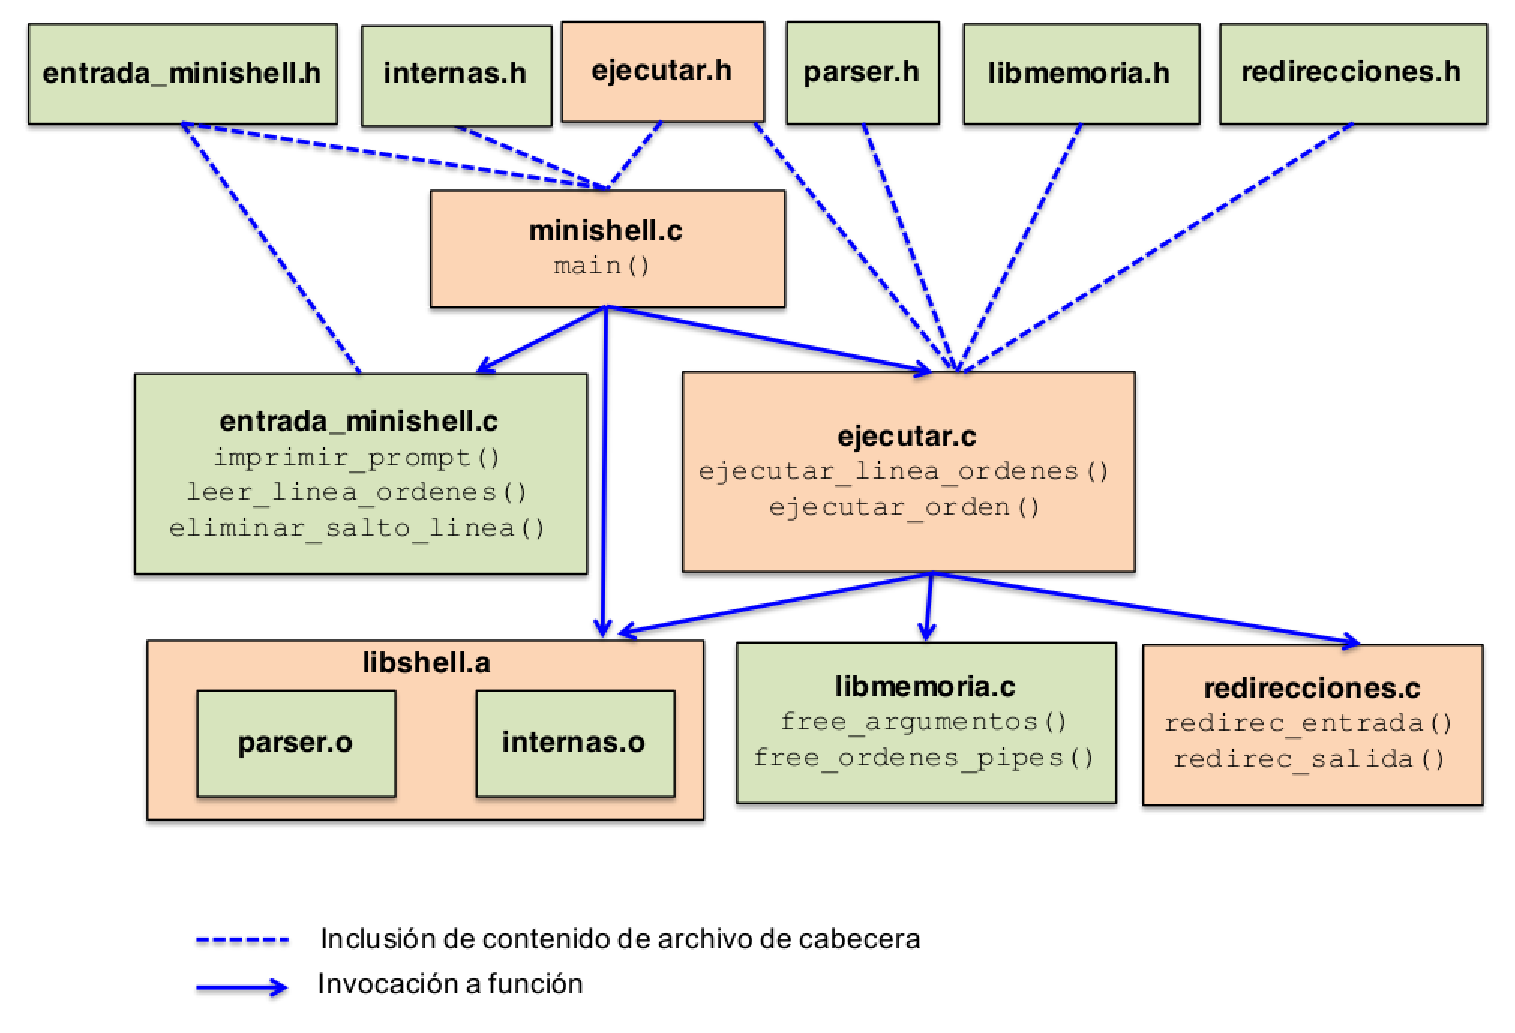
\includegraphics[scale=0.6]{figs/modulosminishell}
\caption{Esquema general de la aplicación \textit{minishell}.}
\label{fig:modulosMinishell}
\end{figure}
\medskip

\end{document}
